\documentclass{book}
\usepackage[utf8]{inputenc}
\usepackage[T1]{fontenc}
\usepackage{lmodern}
\usepackage[a4paper]{geometry}
\usepackage[frenchb]{babel}
\usepackage{graphicx}
\usepackage{hyperref}

\usepackage{pstricks}
\usepackage{pst-node}
\usepackage{wrapfig}

\usepackage{listings}
\lstset{language=C,basicstyle=\scriptsize\color{green},identifierstyle=\color{orange},keywordstyle=\color{blue}}

\usepackage{amsmath}
\usepackage{amssymb}
\bibliographystyle{plain}

\begin{document}
%%%%%%%%%%%%%%%%%%%%%%%%%%%%%%%%%%%%%%%%%%%%%%%%%%%%%%%%%%%%%%%%%%%%%%%%%%%%%%%%%%%%%%%%%
%=======================================================================================%
%%%%%%%%%%%%%%%%%%%%%%%%%%%%%%%%%%%%%%%%%%%%%%%%%%%%%%%%%%%%%%%%%%%%%%%%%%%%%%%%%%%%%%%%%
\begin{titlepage}
%%%%%%%%%%%%%%%%%%%%%%%%%%  LOGO  %%%%%%%%%%%%%%%%%%%%%%%%%%%%%%%%%%%%%%%%%
 \begin{pspicture}(-5,4)(5,5)
%\rput(-5,3){\href{http://www.upmc.fr/FR/info/00}{
\includegraphics[scale=1.0]{upmc_logo}}}
\rput(-4,6.5){
\includegraphics[scale=1.0]{upmc_logo}}
\rput(-4,5){\resizebox{6cm}{0.3cm}{\begin{tabular}{l}
		Université de Pierre et Marie CURIE (PARIS VI) \\
		4 Place Jussieu 75005 Paris
            \end{tabular}}}
%\psline(-5,0)(5,0)
\end{pspicture}
%%%%%%%%%%%%%%%%%%%%%%%%%%  LOGO  %%%%%%%%%%%%%%%%%%%%%%%%%%%%%%%%%%%%%%%%%
%%%%%%%%%%%%%%%%%%%%%%%%%%  Titre %%%%%%%%%%%%%%%%%%%%%%%%%%%%%%%%%%%%%%%%%
\begin{center}
\resizebox{14cm}{1cm}{\bsc{Écoulement laminaire dans une conduite}}\\ 
\large\bsc{équation de Navier-Stokes stationnaire}\\
\large\textbf{Enseigné par M.Frédéric Hecht}
\end{center}
%%%%%%%%%%%%%%%%%%%%%%%%%%  Titre  %%%%%%%%%%%%%%%%%%%%%%%%%%%%%%%%%%%%%%%%%
%%%%%%%%%%%%%%%%%%%%%%%%%%  image maillage %%%%%%%%%%%%%%%%%%%%%%%%%%%%%%%%
\begin{pspicture}(-7,-2)(7,2)
\psline[linecolor=blue](5,1)(-5,1)%Label = 2
\rput(0,1.25){\Rnode{C}{\small{\color{blue}label=2}}}
\psline[linecolor=red](-5,1)(-5,0)%Label = 1
\rput(-5,1.25){\small $\beta$} \rput(-5,-0.25){\small $\alpha$}
\rput{90}(-5.25,0.5){\Rnode{D}{\small{\color{red}label=1}}}
\psline[linecolor=blue](-5,0)(-3,0)(-3,-1)(5,-1)%Label = 2
\rput(0,-1.25){\Rnode{E}{\small{\color{blue}label=2}}}
\pscurve[linecolor=green](5,-1)(4.75,-0.5)(5.1,0)(4.5,0.5)(5,1)%Label = 3
\rput{-90}(5.5,0){\Rnode{F}{\small{\color{green}label=3}}}


\pscurve[linecolor=red](-5,0)(-4,0.5)(-5,1)%Label = 3
\rput(-4.75,0.75){\Rnode{A}{}}
\rput(-6,1.9){\Rnode{B}{\color{red}\small 4*(y-$\alpha$)*($\beta$-y)}}
\ncline{->}{A}{B}

%\psline(-7,-2)(7,2)
\end{pspicture}
%%%%%%%%%%%%%%%%%%%%%%%%%%  image maillage %%%%%%%%%%%%%%%%%%%%%%%%%%%%%%%%%%%%
%%%%%%%%%%%%%%%%%%%%%%%%%%  Auteur %%%%%%%%%%%%%%%%%%%%%%%%%%%%%%%%%%%%%%%%%
\begin{flushright}
\underline{\textbf {NGUYEN Chi Thanh}} \\
{\textbf {2008-2009}}
\end{flushright}
%%%%%%%%%%%%%%%%%%%%%%%%%%  Auteur %%%%%%%%%%%%%%%%%%%%%%%%%%%%%%%%%%%%%%%%%
\begin{center}
\begin{pspicture}(-7,-4)(7,4)
\rput(-3,-5){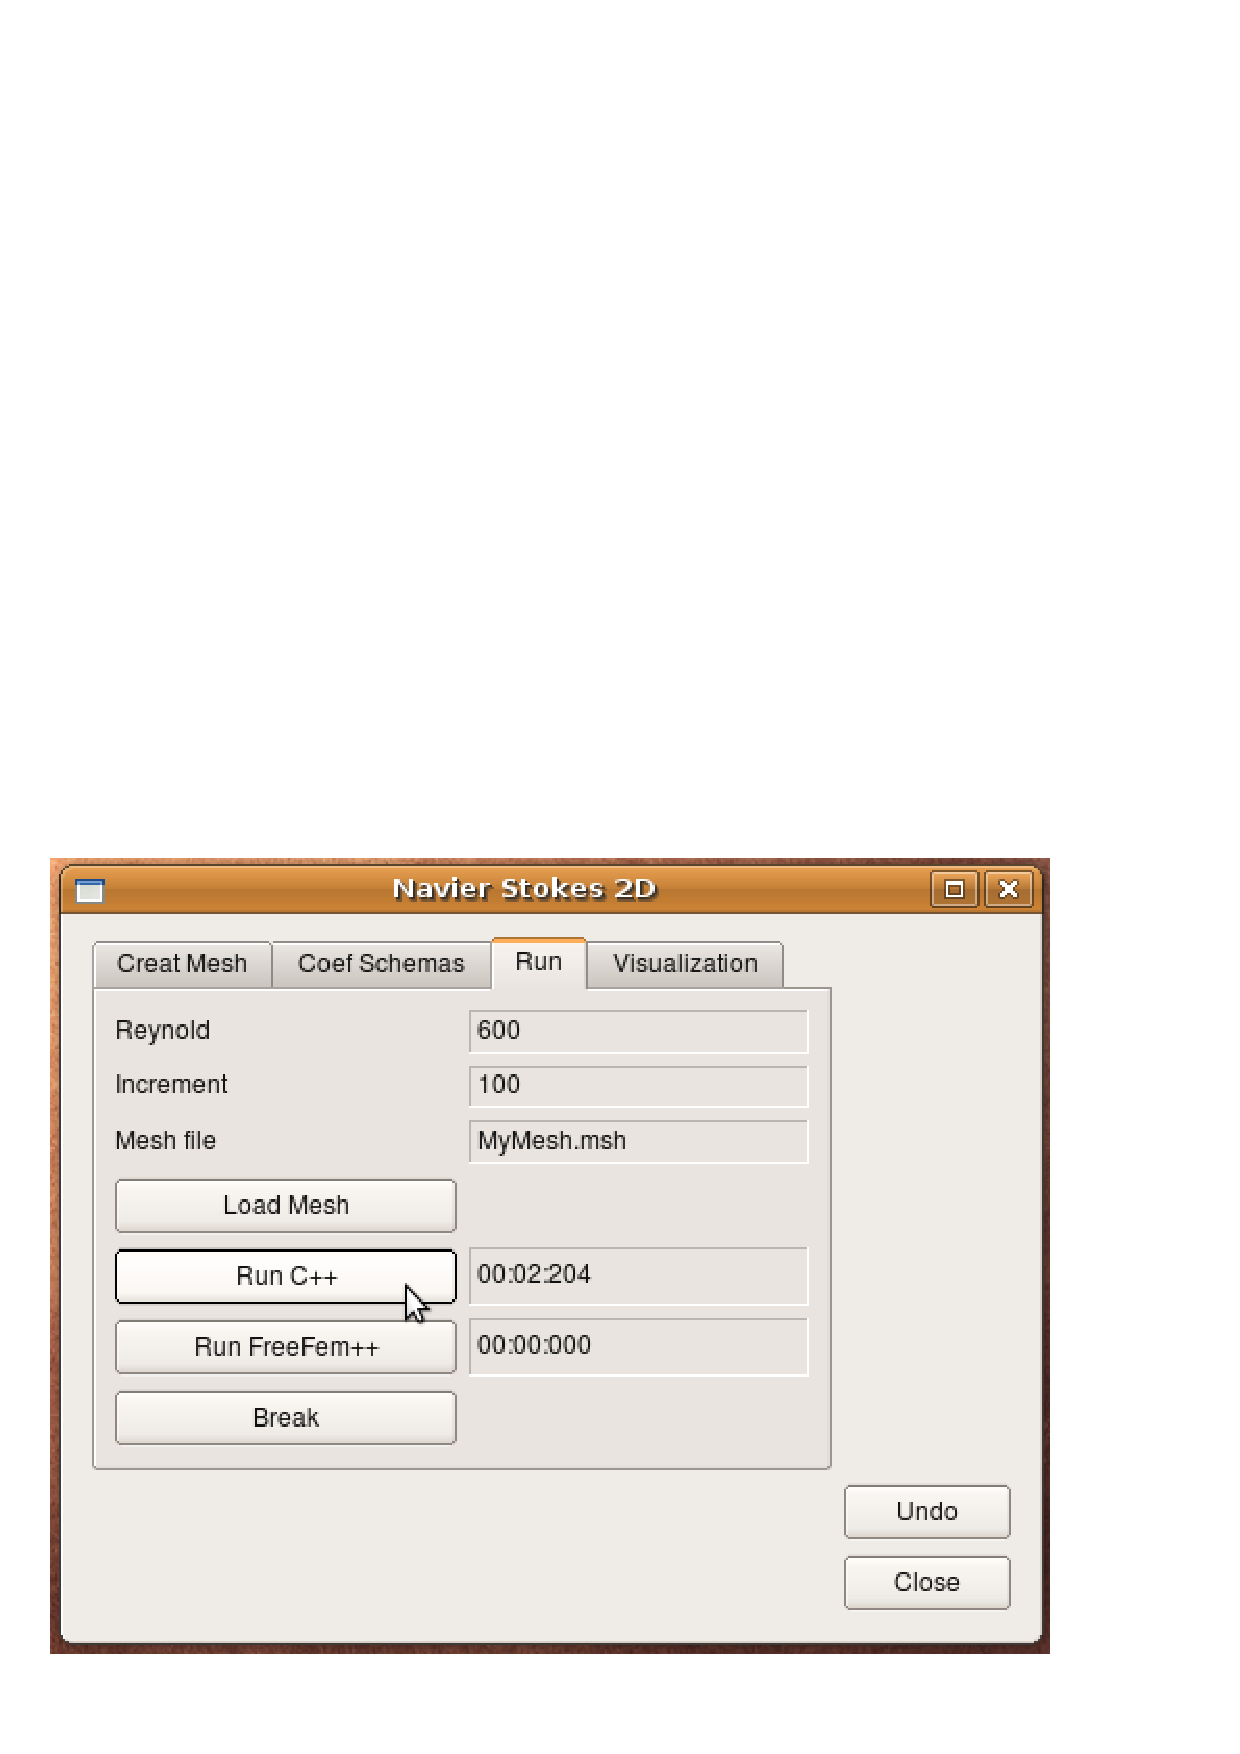
\includegraphics[scale=0.5]{ImageTitle}}
\rput(4.7,3){\begin{tabular}{l}
		$\bullet$  \texttt{Existence et unicité} \\
		$\bullet$  \texttt{Méthode de continuation} \\
		$\bullet$  \texttt{Programmation C++} \\
		$\bullet$  \texttt{Qt Programmation GUI} 	
               \end{tabular}}
%\psline(-7,-4)(7,7)
\end{pspicture}
\end{center}

\end{titlepage}
\tableofcontents
%%%%%%%%%%%%%%%%%%%%%%%%%%%%%%%%%%%%%%%%%%%%%%%%%%%%%%%%%%%%%%%%%%%%%%%%%%%%%%%%%%%%%%%%%
%=======================================================================================%
%%%%%%%%%%%%%%%%%%%%%%%%%%%%%%%%%%%%%%%%%%%%%%%%%%%%%%%%%%%%%%%%%%%%%%%%%%%%%%%%%%%%%%%%%
\chapter*{Introduction}
Dans le cadre des études de Master 2 de mathématique de la modélisation (ANEDP) �  l'université Pierre et Marie Curie, les étudiants suivant le module NM406 (Résolution des EDP par la Méthode des Éléménts Finis) enseigné par \href{http://www.ann.jussieu.fr/~hecht/}{M.Frédéric Hecht} doivent réaliser un projet de calcul scienfique utilisant la FEM développé en C++.Ce projet est basé sur la bibliothèque servant �  développer le logiciel \href{http://www.freefem.org/ff++/}{FreeFem++} par le professeur.  

\paragraph{Phénomène physique : }Le projet consiste �  simuler l'écoulement laminaire dans une conduite en résolvant l'équation de Navier-Stokes stationnaire. Un écoulement laminaire est régulier (il ne présente pas trop de variations spatiales ou temporelles), bien souvent stationnaire.  La viscosité stabilise et régularise les écoulements de façon générale. Un fluide présentant une viscosité importante s'écoulera de façon laminaire. Un écoulement est caractérisé par son nombre de Reynolds, qui permet de se faire une idée de sa stabilité : quand ce nombre est petit, l'écoulement est laminaire, quand il est grand, l'écoulement est en générale instable et turbulent. La transition entre les écoulements stables et instable voire turbulents est un sujet d'étude important. Dans une conduite, on considère souvent que la transition peut se produire entre 2000 et 3000.

\paragraph{Problème mathématique :}Il s'agit en fait d'une solution stable des équations de Navier-Stokes, au sens où si on modifie l'écoulement, il retourne vers la solution laminaire. Le domaine étudié ici est l'un des problème classique : la marche descendante. 
\begin{center}
 \begin{pspicture}(-7,-1.5)(7,1.5)
 \psline[linecolor=blue](5,1)(-5,1)
 \psline[linecolor=red](-5,1)(-5,0)
 \rput(-5.25,0.5){\color{red}$\Gamma$}
 \psline[linecolor=blue](-5,0)(-3,0)(-3,-1)(5,-1)
 \pscurve[linecolor=green](5,-1)(4.75,-0.5)(5.1,0)(4.5,0.5)(5,1)
 \pscurve[linecolor=red](-5,0)(-4,0.5)(-5,1)

 %\psline(-7,-1.5)(7,1.5)
 \end{pspicture}
\end{center}
La conduite horizontale, la rentrée du fluid �  droite avec le profit parabolique représantant la condition Poiseuille donnant le problème mathématique suivant :
\[
(\wp)\hspace{0.25cm}\left\{
\begin{array}{rl}
(\textbf{u}.\triangledown) \textbf{u} -\nu \bigtriangleup \textbf{u} + \triangledown p & =0 \\
\triangledown \textbf{u} & =0 \\
\textbf{u}_\Gamma &=g 
\end{array}\right.
\]
Ayanat pour but de résoudre ce problème,le projet se compose donc l'étude mathématique (existence et l'unicité de solution, l'implémentation numérique), et l'étude informatique basé sur la programmation C++ pour résoudre ce problème.  
%%%%%%%%%%%%%%%%%%%%%%%%%%%%%%%%%%%%%%%%%%%%%%%%%%%%%%%%%%%%%%%%%%%%%%%%%%%%%%%%%%%%%%%%%
%=======================================================================================%
%%%%%%%%%%%%%%%%%%%%%%%%%%%%%%%%%%%%%%%%%%%%%%%%%%%%%%%%%%%%%%%%%%%%%%%%%%%%%%%%%%%%%%%%%
\chapter{Études mathématiques}
Cause de la limite du temps l'étude du cadre fonctionnelle ne sera pas toute détaillée dans ce projet. Ce rapport ne présente qu'une partie briève de l'étude fonctionnelle de l'équation Navier-Stokes dans ce cas concret pour arriver �  l'implémentation informatique, qui est l'essentiel de l'exercice. Pour plus de détails sur la méthode de continuation, il est de préférence de consulter \cite[Girault-Raviart p.297-365]{NCT1} 
\section{Cadre fonctionnelle}
Ce paragraphe montre brièvement la méthode de continuation servant d'une part �  prouver l'existence et l'unicité de la solution, d'autre amener �  l'implémentation du schéma numérique de type Newton. 
\paragraph{Méthode de continuation :} Cette méthode, par la construction d'une fonctionnelle $F$ d'un certain d'espace de départ et d'espace d'arrivé :
\[
\begin{array}{rl}
 \Lambda \times X &\longmapsto \chi \\
 (\lambda,u) &\longmapsto F(\lambda,u)
\end{array}
\]
on peut prouver que la résolution du problème : 
\begin{equation}\label{Pcontinuation}
 F(\lambda,u)=0
\end{equation}
est équivalent au problème : 
\begin{equation}\label{Pnavierstokes}
(\wp)\hspace{0.25cm}\left\{
\begin{array}{rl}
(\textbf{u}.\triangledown) \textbf{u} -\nu \bigtriangleup \textbf{u} + \triangledown p & =0 \\
\triangledown \textbf{u} & =0 \\
\textbf{u}_\Gamma &=g 
\end{array}\right.
\end{equation}
Pour comprendre ce mécanisme, on a besoin de quelques définitions des espaces fonctionnelles et ses opérateurs :
\paragraph{Espaces fonctionnels :}
\[
\begin{array}{rl}
  I & \subset \Re \\
  X & =H^1(\Omega)^N \times L^2_0(\Omega)\\
  Y & =H^{-1}(\Omega)^N \times \{ g \in H^{\frac{1}{2}}(\Gamma)^N, \int_{\partial\Omega}g.nd\sigma=0 \}
\end{array}
\]
\paragraph{Opérateur de Stokes :}
Soit le problème de Stokes :
\[
\left\{
\begin{array}{rl}
(-\nu \bigtriangleup \textbf{u} + \triangledown p & =f \\
\triangledown \textbf{u} & =0 \\
\textbf{u}_\Gamma &=g 
\end{array}\right.
\]
On peut démontrer l'existence et l'unicité de ce problème dans $X$. De sorte que l'on peut définir un isomorphisme :
\[T : 
\begin{array}{rl}
Y &\longmapsto X \\
 \left[\begin{array}{ll}f\\g\end{array}\right] &\longmapsto \left[\begin{array}{ll}u\\p\end{array}\right]
\end{array}
\]
Remarque : T est linéaire, continue donc différentialble.
\paragraph{Opérateur auxiliaire :}
On définit encore un autre opérateur :
\[G : 
\begin{array}{rl}
I \times X &\longmapsto Y \\
 ( \lambda, \left[\begin{array}{ll}v\\q\end{array}\right] ) &\longmapsto -\left[\begin{array}{cc}\lambda(f-(v.\triangledown)v)\\g\end{array}\right]
\end{array}
\]
On peut remarquer encore que l'application partielle $G(\lambda,.)$ est linéaire continue, donc il est facile �  calculer sa différentielle. 
\paragraph{Opérateur de continuation :}
On s'amène finalement �  définir l'opérateur $F=Id +T \circ G$, c'est �  dire :
\[F : 
\begin{array}{rl}
I \times X &\longmapsto X \\
 ( \lambda, \left[\begin{array}{ll}u\\p\end{array}\right] ) &\longmapsto 
 F( \lambda, \left[\begin{array}{ll}u\\p\end{array}\right] )
 =Id\left[\begin{array}{ll}u\\p\end{array}\right] 
 +T\circ G ( \lambda, \left[\begin{array}{ll}u\\p\end{array}\right] ) 
\end{array}
\]
De sorte que comme G, $F(\lambda,.)$ est une application linéaire continue de $X$ �  $Y$, que l'on peut calculer facilement la différentielle de cettet application partielle : 
\[F(\lambda,\bullet) : 
\begin{array}{rl}
 X &\longmapsto X \\
 \left[\begin{array}{ll}u\\p\end{array}\right] &\longmapsto 
 Id\left[\begin{array}{ll}u\\p\end{array}\right] 
 +T\circ G ( \lambda, \left[\begin{array}{ll}u\\p\end{array}\right] ) 
\end{array}
\]
Partant de ces principales constructions d'espaces et opérateurs, en utilisant ensuite la théorie des fonctions implicites, on se ramène �  prouver l'équivalent des problème ~\eqref{Pcontinuation} et ~\eqref{Pnavierstokes}. L'étude fonctionnelle prouve que $\left[\begin{array}{ll}u\\p\end{array}\right]$ de $X$ est solution du problème ~\eqref{Pnavierstokes} si et seulement si $\left[\begin{array}{ll}u\\ \frac{p}{\nu}\end{array}\right]$ de $X$ est solution du problème $F(\frac{1}{\nu},\bullet)=0$.
\section{Cadre numérique}
Issu de la conclution de la dernière section, on peut utiliser le schéma de Newton pour résoudre le problème $F(\frac{1}{\nu},\bullet)=0$. Soit $\left[\begin{array}{ll}u\\ \frac{p}{\nu}\end{array}\right]$ solution, par le théorème d'inversion local, on a :
\[
F(\lambda,\left[\begin{array}{ll}u\\ \frac{p}{\nu}\end{array}\right])=0 \Longleftrightarrow
\partial_{up}F_{(u,p)}(\frac{1}{\nu},\bullet) \text{est un isomorphisme}.
\]
Pour la résolution numérique, on peut utiliser le schéma de Newton :
\[
\left[\begin{array}{ll}u^{n+1}\\ \frac{p^{n+1}}{\nu}\end{array}\right]=
\left[\begin{array}{ll}u^{n}\\ \frac{p^{n}}{\nu}\end{array}\right]-
\partial_{up}F^{-1}_{(u^n,\frac{p^n}{\nu})}(\frac{1}{\nu},\bullet) \circ
F(\frac{1}{\nu},\left[\begin{array}{ll}u^{n}\\ \frac{p^{n}}{\nu}\end{array}\right])
\]
En calculant la différentielle de $F$ par les différentielles de $G$ et de $T$, on arrive au :
\paragraph{Schéma de Newton :}
\[
(N)\hspace{0.25cm}\left\{
\begin{array}{rl}
-\bigtriangleup \textbf{u}^{n+1} + \frac{1}{\nu}[( \textbf{u}^n. \triangledown) \textbf{u}^{n+1}+ (\textbf{u}^{n+1} .\triangledown) \textbf{u}^n] + \triangledown p^{n+1} &=\frac{1}{\nu}(\textbf{u}^n.\triangledown)\textbf{u}^n \\
\text{div}\textbf{u}^{n+1}          &=0 \\
\textbf{u}^{n+1}_{|\Gamma_D}  &=g
\end{array}\right.
\]
Partant de ce schémas, en affectant que $\textbf{uold}=\textbf{u}^{n}$ est la solution calculée de l'itération précédante, $\textbf{u}=\textbf{u}^{n+1}$ est la solution �  calculer, on récrit pour chaque itération, le problème devient : 
\[
(N)\hspace{0.25cm}\left\{
\begin{array}{rl}
-\bigtriangleup \textbf{u} + \frac{1}{\nu}[( \textbf{uold}. \triangledown) \textbf{u}+ (\textbf{u} .\triangledown) \textbf{uold}] + \triangledown p &=\frac{1}{\nu}(\textbf{uold}.\triangledown)\textbf{uold} \\
\text{div}\textbf{u}          &=0 \\
\textbf{u}_{|\Gamma_D}  &=g
\end{array}\right.
\]
Soit $\left[\begin{array}{cc} \textbf{v}\\ q\end{array}\right]$ dans le même espace, en multipliant et intégrant, le problème équivalent �  la :
\paragraph{Formulation Variationnelle :}
\[
\left\{
\begin{array}{rl}
-\int_{\Omega} \bigtriangleup \textbf{u.v} + 
\frac{1}{\nu}\int_{\Omega} [( \textbf{uold}. \triangledown) \textbf{u}+ (\textbf{u} .\triangledown) \textbf{uold}].\textbf{v}  &\\
+\int_{\Omega} \triangledown p.\textbf{v}
-\int_{\Omega} q\text{div}\textbf{u} &=
\frac{1}{\nu}\int_{\Omega}(\textbf{uold}.\triangledown)\textbf{uold}.\textbf{v} \\
\textbf{u}_{|\Gamma_D}  &=g
\end{array}\right.
\]
En développant terme �  terme de la première égalité, on a :
\[
\begin{array}{rl}

-\int_{\Omega} \bigtriangleup \textbf{u.v} &=\int_{\Omega} \triangledown \textbf{u}.\triangledown \textbf{v}\color{blue}{-\int_{\partial\Omega} \bigtriangleup \textbf{u}.(\textbf{v}.\textbf{n})\text{d}\sigma}\\
 
+\frac{1}{\nu}\int_{\Omega} [( \textbf{uold}. \triangledown) \textbf{u}+ (\textbf{u} .\triangledown) \textbf{uold}].\textbf{v} &=+\frac{1}{\nu}\int_{\Omega} [( \textbf{uold}. \triangledown) \textbf{u}+ (\textbf{u} .\triangledown) \textbf{uold}].\textbf{v} \\

+\int_{\Omega} \triangledown p.\textbf{v} &=-\int_{\Omega} p\text{div}\textbf{v}\color{blue}{+\int_{\partial\Omega} p.(\textbf{v}.\textbf{n})\text{d}\sigma}\\
 
-\int_{\Omega} q\text{div}\textbf{u} &=-\int_{\Omega} q\text{div}\textbf{u}\\

\frac{1}{\nu}\int_{\Omega}(\textbf{uold}.\triangledown)\textbf{uold}.\textbf{v}&=\frac{1}{\nu}\int_{\Omega}(\textbf{uold}.\triangledown)\textbf{uold}.\textbf{v} 
\end{array}
\]
Avec la condition de sortie $\color{blue}{-\int_{\partial\Omega} \bigtriangleup \textbf{u}.(\textbf{v}.\textbf{n})\text{d}\sigma}=\color{blue}{+\int_{\partial\Omega} p.(\textbf{v}.\textbf{n})\text{d}\sigma}$ il reste donc la formulation variationnelle pour une itération : 
\[
\left\{
\begin{array}{rl}
\int_{\Omega} \triangledown \textbf{u}.\triangledown \textbf{v}
+\frac{1}{\nu}\int_{\Omega} [( \textbf{uold}. \triangledown) \textbf{u}+ (\textbf{u} .\triangledown) \textbf{uold}].\textbf{v} &\\ 

-\int_{\Omega} p\text{div}\textbf{v}
 
-\int_{\Omega} q\text{div}\textbf{u} &=

 \frac{1}{\nu}\int_{\Omega}(\textbf{uold}.\triangledown)\textbf{uold}.\textbf{v}\\
\textbf{u}_{|\Gamma_D}  &=g 
\end{array}
\right.
\]
Le dernier travail de l'étude numérique est donc définir les espaces discrets. Soit le domaine de calcul $\Omega$, $\partial\Omega$ est la partie du bord de domaine dont la vitesse s'annule. Plusieurs choix sont possible, mais dans ce projet, on travail avec un exemple qui marche très bien dans ce cas, l'élement fini de type Taylor-Hood (P1-P2). On définit les espaces :
\[
\begin{array}{rl}
X_h &= \left\{ \textbf{v}\in C^0(\overline{\Omega})^d; \textbf{v}_{|\kappa}\in \text{P}^d_2 \hspace{0.5cm} \forall \kappa \in T_h, \textbf{v}_{|\partial\Omega}=0 \right\}         \\

M_h &= \left\{ q\in C^0(\overline{\Omega});q_{|\kappa}\in \text{P}_1 \hspace{0.5cm} \forall \kappa \in T_h \right\}\cap\text{L}^2_0(\Omega) 
\end{array}
\]
\paragraph{Le problème discret :}La question qui se pose dans le cadre discret est donc trouver $\left[\begin{array}{cc} \textbf{u}\\ p\end{array}\right] \in X_h \times M_h$ tels que $\forall \left[\begin{array}{cc} \textbf{v}\\ q\end{array}\right] \in X_h \times M_h$, on a : 

\[
\left\{
\begin{array}{rl}
\int_{\Omega} \triangledown \textbf{u}.\triangledown \textbf{v}
+\frac{1}{\nu}\int_{\Omega} [( \textbf{uold}. \triangledown) \textbf{u}+ (\textbf{u} .\triangledown) \textbf{uold}].\textbf{v} &\\ 

-\int_{\Omega} p\text{div}\textbf{v}
 
-\int_{\Omega} q\text{div}\textbf{u} &=

 \frac{1}{\nu}\int_{\Omega}(\textbf{uold}.\triangledown)\textbf{uold}.\textbf{v}\\
\textbf{u}_{|\Gamma_D}  &=g 
\end{array}
\right.
\]

\section{Reynold}
La résolution de l'équation de Navier-Stokes a été toujours difficile pour les nombres de Reynolds très grand, qui représente le rapport entre les forces d'inertie et les forces visqueuses. Si le nombre de Reynolds est très grand, l'équation devient fortement non-linéaire car les phénomènes convectifs dominent. Les non-linéarités produiront des effets instationnaires pour un forçage stationnaire, des brisures de symétries par rapport aux conditions aux limites initiales, en d'autre termmes la turbulence, qui explose le système. 

La méthode adopte donc une stratégie qui résoud l'équation en auguementant le nombre de Reynolds petit �  petit. Soit la solution $\textbf{u}_{REY}$ correspond au nombre de Reynolds=REY, on résoud le système en retrouvant les solutions $\textbf{u}_{rey}$ correspond �  $rey < REY$, et puis on augemente $rey$ pour atteindre $REY$. L'algorithme est :
\[
\left\{
\begin{array}{lll}
\text{while } (rey<REY \hspace{0.25cm}) \\
\hspace{0.5cm} \{ \\
\hspace{1cm}\text{while }(\| \textbf{u}-\textbf{uold})\| \geqslant 10^{-6})\\
\hspace{1.5cm}\text{Résoudre }\textbf{u}= \textbf{uold}-\text{dF}^{-1}_{\textbf{uold}}(\text{F}(\textbf{uold}));\\
\hspace{1cm}rey+=incrementRey; \\
\hspace{0.5cm} \} 
\end{array}
\right.
\]
Dans ce projet, particulièrement dans ce programme en C++ et son domaine de calcul (La marche descendante), la résolution peut atteindre Reynolds=1400 pour les auguementations de 50 ou 100, partant de Reynolds=1.
%%%%%%%%%%%%%%%%%%%%%%%%%%%%%%%%%%%%%%%%%%%%%%%%%%%%%%%%%%%%%%%%%%%%%%%%%%%%%%%%%%%%%%%%%
%=======================================================================================%
%%%%%%%%%%%%%%%%%%%%%%%%%%%%%%%%%%%%%%%%%%%%%%%%%%%%%%%%%%%%%%%%%%%%%%%%%%%%%%%%%%%%%%%%%
\chapter{Études informatiques}
\section{Création de maillage}
Comme présenté, le domaine de calcul est une marche descendante de la forme :
%%%%%%%%%%%%%%%%%%%%%%%%%%  image Mesh%%%%%%%%%%%%%%%%%%%%%%%%%%%%%%%%%%%%%%%%%
\begin{center}
\begin{pspicture}(-7,-1.5)(7,1.5)
\psline[linecolor=blue](5,1)(-5,1)%Label = 2
\rput(0,1.25){\Rnode{C}{\small{\color{blue}label=2}}}
\psline[linecolor=red](-5,1)(-5,0)%Label = 1
\rput(-5,1.25){\small $\beta$} \rput(-5,-0.25){\small $\alpha$}
\rput{90}(-5.25,0.5){\Rnode{D}{\small{\color{red}label=1}}}
\psline[linecolor=blue](-5,0)(-3,0)(-3,-1)(5,-1)%Label = 2
\rput(0,-1.25){\Rnode{E}{\small{\color{blue}label=2}}}
\pscurve[linecolor=green](5,-1)(4.75,-0.5)(5.1,0)(4.5,0.5)(5,1)%Label = 3
\rput{-90}(5.5,0){\Rnode{F}{\small{\color{green}label=3}}}


\pscurve[linecolor=red](-5,0)(-4,0.5)(-5,1)%Label = 3
\rput(-4.75,0.75){\Rnode{A}{}}
\rput(-6,1.5){\Rnode{B}{\color{red}\small 4*(y-$\alpha$)*($\beta$-y)}}
\ncline{->}{A}{B}

%\psline(-7,-1.5)(7,1.5)
\end{pspicture}
\end{center}
%%%%%%%%%%%%%%%%%%%%%%%%%%  image Mesh %%%%%%%%%%%%%%%%%%%%%%%%%%%%%%%%%%%%%%%%%

Les degré de liberté setrouvant sur le label1 seront affectées par la condition de Dirichelet qui forme un profil parabolique de fluid entré. Sur le label2 la vitesse sera null. Sur le label3, les termes sont considéré comme l'intérieur du domaine (sont �  calculer).
\paragraph{Création de Maillage : }
La création de maillage se fait par Freefem++, en utilisant le script : CreatMesh.edp. Ce script lit les données dans le fichier MeshCorner.txt contenant les trois coins du maillage et un coeficient indiquant la densité de noeuds pour le maillage. En l'éxécutant, il crée un fichier MyMesh.msh contenant les données de maillage, fait une visualisation de maillage créé. 
\begin{lstlisting}
prompt$FreeFem++ CreatMesh.edp 
\end{lstlisting}
%%%%%%%%%%%%%%%%%%%%%%%%%%%%%%%%%%%%%%%%%%%%%%%%%%%%%%%%%%%%%%%%%%%%%%%%%%%%%%%%%
\section{Conditions de bord}
La stratégie pour affecter la condition de Dirichelet au bord sur le label1 est :
\[
\left\|
\begin{array}{l}
\text{parcourir les arrêtes au bord} \\
\hspace{0.2cm} \{ \\
\hspace{0.4cm} \text{Trouver l'élément fini qui contient l'arrête;}\\
\hspace{0.4cm} \text{Parcourir les df locale} \\
\hspace{0.6cm} \{ \\
\hspace{0.8cm} \text{Si ((Label==1) et (df est sur l'arrête))} \\
\hspace{1cm}   \{ \\
\hspace{1.2cm}     \text{affecter la condition de bord au vecteur global;} \\
\hspace{1cm}   \} \\
\hspace{0.6cm} \} \\
\hspace{0.2cm} \}
\end{array}
\right.
\]
Donc l'implémentation dans C++ est :
\begin{lstlisting}[language=C]
for (int ke=0;ke<Th.nbe;ke++){
 int kf,k=Th.BoundaryElement(ke,kf);
 FElement FK(Vh[k]);
 int nbdf=FK.NbDoF();
 int Label=Th.borderelements[ke].lab;
 for (int df =0;df<nbdf;++df){//condition Dirichelet
  if(((Element::onWhatBorder[kf][FK.DFOnWhat(df)])!=0)&&(Label==1)){
    int p=FK.DFOnWhat(df);Rd P(FK.pPi_h(p));
    dirichelet[FK(df)]=Poissieulle(P,FK.FromASubFE(df)); 
    }	
  }
}
\end{lstlisting}
Ensuite pour la résolution linéaire générale, on a une méthode de très grande valeur (TGV) servant �  résoudre le système de type Ax=b excepté de quelques points du vecteur x :
\[
\begin{array}{cc}
\left[
\begin{array}{lllll}
{\color{red}\bullet} & & & &\\
 & & & &\\
 & & & &\\
 & & &{\color{red}\bullet} &\\
 & & & &
\end{array}
\right]
\\
A
\end{array}
\begin{array}{cc}
\left[
\begin{array}{lllll}
{\color{blue}\bullet}\\
\\
\\
{\color{blue}\bullet}\\
\\
\end{array}
\right]
\\
x
\end{array}
=
\begin{array}{cc}
\left[
\begin{array}{lllll}
{\color{red}\bullet}\\
\\
\\
{\color{red}\bullet}\\
\\
\end{array}
\right]
\\
b
\end{array}
\]
Sur la matrice A, les points rouges sont sur la diagonale, de même lignes que ceux du vecteur b. En mutipliant les points rouges par une valeur très très grande (de l'ordre de $10^{30}$) avant de résoudre le système, après la résolution, les points bleus prendront la même valeur que les points rouge du vecteur b avant de mutiplication. L'implémentation du code de cette méthode est suivant :
\begin{lstlisting}
for(int ke=0;ke<Th.nbe;++ke){	
 int kf,k=Th.BoundaryElement(ke,kf);
 FElement FK(Vh[k]);
 int ndf=FK.NbDoF();int Label=Th.borderelements[ke].lab;
  for (int df =0;df<ndf;++df){
  if (Element::onWhatBorder[kf][FK.DFOnWhat(df)] && (Label!=3)){
   if(FK.FromASubFE(df) < d){
    int i=FK(df);
    A[make_pair(i,i)] = tgv;
    b[i] = tgv*dirichelet[i];
    kkk++;
   }
  }
 }  
}
\end{lstlisting}
%%%%%%%%%%%%%%%%%%%%%%%%%% PASSAGE LOCAL-GLOBALE %%%%%%%%%%%%%%%%%%%%%%%%%%%%%%%%
\section{Passage Locale-Globale}
L'idée fondamentale du problème est �  partir de la formulation variationnelle, on doit construire un système linéaire �  résoudre. La question est comment construire ce système linéaire dans le cadre général. Cette question se pose sur un principe basique : le passage local-globale. Soit, l'espace fonctionnel discret $X_h \times M_h$ (FESpace) qui se construit par le maillage (Mesh) et le type d'élément fini (TypeOfFE). Un FESpace se compose aussi des FElement, qui décrit toutes les données dans un élément fini. Une fonction discrète dans FESpace est caractérisée par ses NBOFDF degré de liberté (NBOFDF est le nombre de degrée de liberté globale), localement, elle est caractérisé par ses nbofdf degré de liberté (nbofdf est le nombre de degré de liberté locale). L'algorithme pour toute opération sur les fonctions est dont de parcourir les FElement, effectuer les opérations sur les df locale, rassembler les résultat par le passage ses df au DF (degré de liberté global). En supposant que l'on a construit une matrice locale ML, le passage �  la matrice M globale se fait par :
\begin{lstlisting}
for(int i=0;i<nbDoF;i++)//Local==>GLOBALE 
  for(int j=0;j<nbDoF;j++) 
    M[make_pair<int,int>(FK(i),FK(j))] +=ML(i,j) ; 
\end{lstlisting}
Il en est de même pour les vecteurs. Supposont que le vecteur local VL a été construit, le passage au vecteur b global se fait par :
\begin{lstlisting}
for(int idf=0;idf<nbDoF;idf++) 
  b[FK(idf)]+=VL[idf];
\end{lstlisting}
%%%%%%%%%%%%%%%%%%%%%%%%%% PASSAGE LOCAL-GLOBALE %%%%%%%%%%%%%%%%%%%%%%%%%%%%%%%%

%%%%%%%%%%%%%%%%%%%%%%%%%% PASSAGE GLOBALE LOCALE%%%%%%%%%%%%%%%%%%%%%%%%%%%%%%%%
\section{Passage Global-Local}
Cette étape est necessaire dans le cas où le schéma est itératif, utilise les valeurs de la solution calculé de l'itération précédante pour calculer la solution après. C'est l'étape sachant une fonction $UOLD$ calculée, comment lire ces valeurs locales, afin de les passer dans le matrice A �  doite et le vecteur b �  gauche pour le système A.X=b. Les valeurs necessaires ne sont pas exactement les df de $UOLD$ au points d'interpolation, mais ce sont des valeurs de $UOLD$ aux points d'intégration. Pour chaque FElement, on doit donc parcourir les points d'intégration de la méthode d'intégration choisie, retrouver les valeurs necessaires de $UOLD$ sur ces points (valeurs de $UOLD$ et valeur de la dérivée de $UOLD$). Ces valeurs seront stoquées dans un vecteur local $uold$
\begin{lstlisting}
for (int ipq=0;ipq<qf.n;ipq++){//qf.n=7
  /*======Les valeurs de UOLD local=====*/
 for(int ic=0;ic<d;ic++){ 
 uold(ic)=FK(qf[ipq],UOLD,ic,op_id);
   for(int ioperator=0;ioperator<d;ioperator++){
   Duold(ic,ioperator)=FK(qf[ipq],UOLD,ic,op_div[ioperator]);
   }	
 }	 
}
\end{lstlisting}
%%%%%%%%%%%%%%%%%%%%%%%%%% PASSAGE GLOBALE LOCALE%%%%%%%%%%%%%%%%%%%%%%%%%%%%%%%%


%%%%%%%%%%%%%%%%%%%%%%%%%% MATRICE LOCAL %%%%%%%%%%%%%%%%%%%%%%%%%%%%%%%%
\section{Matrice locale}
La construction de la matrice locale est fondamentale dans tout le programme. C'est cette étape qui implémente le schéma de l'algorithme mathématique. Partant le la formulation variationnelle : 
\begin{equation}
\label{Formulation}
\begin{array}{rl}
\int_{\Omega} \triangledown \textbf{u}.\triangledown \textbf{v}
+\frac{1}{\nu}\int_{\Omega} [( \textbf{uold}. \triangledown) \textbf{u}+ (\textbf{u} .\triangledown) \textbf{uold}].\textbf{v} &\\ 

-\int_{\Omega} p\text{div}\textbf{v}
 
-\int_{\Omega} q\text{div}\textbf{u} &=

 \frac{1}{\nu}\int_{\Omega}(\textbf{uold}.\triangledown)\textbf{uold}.\textbf{v}
\end{array}
\end{equation}
On la détaille dans le cas 3D. Dans ce  cas, soit :
\[
\left[
\begin{array}{cc}
\textbf{u} \\
p
\end{array}
\right]
=
\left[
\begin{array}{cccc}
u1 \\
u2 \\
u3 \\
p
\end{array}
\right]
\hbox{,  }
\left[
\begin{array}{cc}
\textbf{v} \\
q
\end{array}
\right]
=
\left[
\begin{array}{cccc}
v1 \\
v2 \\
v3 \\
q
\end{array}
\right]
\hbox{,  }
\left[
\begin{array}{cc}
\textbf{uold} \\
pold
\end{array}
\right]
=
\left[
\begin{array}{cccc}
uold1 \\
uold2 \\
uold3 \\
pold
\end{array}
\right]
\]
La formulation ~\eqref{Formulation} détallée dans le cas 3D sera :
%%%%%%%%%%%%%%%%%%%%%%%%%%%%
\[
\begin{array}{l}
\int_{\Omega}\left[
\begin{array}{c}%Terme grad grad
 \frac{\partial u1}{\partial x}\frac{\partial v1}{\partial x}
+\frac{\partial u1}{\partial y}\frac{\partial v1}{\partial y}
+\frac{\partial u1}{\partial z}\frac{\partial v1}{\partial z} \\
 \frac{\partial u2}{\partial x}\frac{\partial v2}{\partial x}
+\frac{\partial u2}{\partial y}\frac{\partial v2}{\partial y}
+\frac{\partial u2}{\partial z}\frac{\partial v2}{\partial z} \\
 \frac{\partial u3}{\partial x}\frac{\partial v3}{\partial x}
+\frac{\partial u3}{\partial y}\frac{\partial v3}{\partial y}
+\frac{\partial u3}{\partial z}\frac{\partial v3}{\partial z} 
\end{array} \right] \\
+\frac{1}{\nu}\int_{\Omega}\left[
\begin{array}{c}
\left(\begin{array}{c}%terme nonlineaire1
uold1 \frac{\partial u1}{\partial x} v1  +
uold2 \frac{\partial u1}{\partial y} v1  +
uold3 \frac{\partial u1}{\partial z} v1  \\
uold1 \frac{\partial u2}{\partial x} v2  +
uold2 \frac{\partial u2}{\partial y} v2  +
uold3 \frac{\partial u2}{\partial z} v2  \\
uold1 \frac{\partial u3}{\partial x} v3  +
uold2 \frac{\partial u3}{\partial y} v3  +
uold3 \frac{\partial u3}{\partial z} v3  
\end{array}\right)
+
\left(\begin{array}{c}%terme nonlineaire2
u1v1 \frac{\partial uold1}{\partial x}  +
u2v1 \frac{\partial uold1}{\partial y}  +
u3v1 \frac{\partial uold1}{\partial z}  \\
u1v2 \frac{\partial uold2}{\partial x}  +
u2v2 \frac{\partial uold2}{\partial y}  +
u3v2 \frac{\partial uold2}{\partial z}  \\
u1v3 \frac{\partial uold3}{\partial x}  +
u2v3 \frac{\partial uold3}{\partial y}  +
u3v3 \frac{\partial uold3}{\partial z}   
\end{array}\right)
\end{array} \right] \\
-\int_{\Omega}\left[
\begin{array}{c}%pdivv
p\frac{\partial v1}{\partial x} \\
p\frac{\partial v2}{\partial y} \\
p\frac{\partial v3}{\partial z} 
\end{array} \right] \\
-\int_{\Omega}
\begin{array}{c}%qdivu
q\left[ \frac{\partial u1}{\partial x} +
 \frac{\partial u2}{\partial y} +
 \frac{\partial u3}{\partial z} 
 \right]
\end{array}  \\
=\frac{1}{\nu}\int_{\Omega}\left[
\begin{array}{c}%membre droit
uold1 \frac{\partial uold1}{\partial x} v1  +
uold2 \frac{\partial uold1}{\partial y} v1  +
uold3 \frac{\partial uold1}{\partial z} v1  \\
uold1 \frac{\partial uold2}{\partial x} v2  +
uold2 \frac{\partial uold2}{\partial y} v2  +
uold3 \frac{\partial uold2}{\partial z} v2  \\
uold1 \frac{\partial uold3}{\partial x} v3  +
uold2 \frac{\partial uold3}{\partial y} v3  +
uold3 \frac{\partial uold3}{\partial z} v3  
\end{array} \right] 
\end{array}
\]

A rappeler que dans ce cas, l'élément fini utilisé est de type Taylor-Hood (P1-P2), avec dimension 3D, chaque fonction se compose de 3 composantes de vitesse et une composante de presssion. Ce qui découpe la matrice locale en bloque.  
\[
\left\|
\begin{array}{l}
\text{BOUCLE pour chaque FElement} \\
\text{Parcourir les points d'intégration} \\
\text{ Calcul des coef d'intégration;} \\
\text{ parcourir les composantes de la fonctions de solution}\\
\text{   parcourir les composantes de la fonctions de test}\\
\text{      parcourir les df de composante}\\
\text{          rajouter des coeufficients dans la matrice locale;} 
\end{array}
\right.
\]
Pour parcourir les points d'intégrations :
\begin{lstlisting}
for (int ipq=0;ipq<qf.n;ipq++){//qf.n=7
 w=0.;uold=0.;Duold=0.;
 QuadraturePoint Pq(qf[ipq]);
 //les coef pour le schemas general
 R coefadvect= CADVECT*mes* Pq.a;
 R coefgradgrad = CGRADGRAD*mes*Pq.a;
 R coefqdivv = CQDIVV*mes*Pq.a;
 R coefpp =1e-10*mes*Pq.a;
 FK.BF(whatd, Pq,w); 
\end{lstlisting}
Calcul des valeurs locales de $uold$ :
\begin{lstlisting}
for(int ic=0;ic<d;ic++){ 
 uold(ic)=FK(qf[ipq],UOLD,ic,op_id);
 for(int ioperator=0;ioperator<d;ioperator++){
 Duold(ic,ioperator)= FK(qf[ipq],UOLD,ic,op_div[ioperator]);
 }	
}	  
\end{lstlisting}
et pour parcourir les composantes des fonctions et ses df :
\begin{lstlisting}
for(int ic=0;ic<d;ic++){//ic=composante v.
  for(int jc=0;jc<d;jc++){//jc=composante u
  int idfbegin=FK.dfcbegin(ic); int idfend=FK.dfcend(ic); 
  int jdfbegin=FK.dfcbegin(jc); int jdfend=FK.dfcend(jc); 
  ........
\end{lstlisting}
%%%%%%%%%%%%%%%%%%%%%%%%%% MATRICE LOCAL %%%%%%%%%%%%%%%%%%%%%%%%%%%%%%%%

%%%%%%%%%%%%%%%%%%%%%%%% PASSAGE AU MEMBRE DROITE %%%%%%%%%%%%%%%%%%%%%%%%%%
\section{Passage au membre droite}
Dans les cas des schémas itératif, le passage de la solution calculée au memebre �  droite est aussi important et se fait de façon similaire que la construction de la matrice du système A.x=b. Comme la construction de la matrice du système, ce passage necessite en premier la construction locale des valeurs de la fonctions calculée aux points d'intégrations. La construction locale se fait en premier par parcourir localement les composantes de la fonction, puis parcourir les df locales de cette composante : 
\begin{lstlisting}
for(int ic=0;ic<d;++ic){
int dfbegin=FK.dfcbegin(ic),dfend=FK.dfcend(ic);
 for(int i=dfbegin;i<dfend;i++){
   for(int i_derivate=0;i_derivate<d;i_derivate++){
      //(uold.grad)uold.vi
      VL[i] +=coefadvec*uold(i_derivate)
              *Duold(ic,i_derivate)*w(i,ic,op_id);
   }
 }
}
\end{lstlisting}
Après chaque calcul local, il ne reste �  faire l'implément dans le vecteur global :
\begin{lstlisting}
..........
   for(int idf=0;idf<nbDoF;idf++) 
      b[FK(idf)]+=VL[idf];
............
\end{lstlisting}
%%%%%%%%%%%%%%%%%%%%%%%% PASSAGE AU MEMBRE DROITE %%%%%%%%%%%%%%%%%%%%%%%%%%
%%%%%%%%%%%%%%%%%%%%%STRUCTURE ET UTILISATION %%%%%%%%%%%%%%%%%%
\section{Structure du programme et utilisation}
Les programmes de calcul est codé en C++. Quelques script de FreeFem++ sont programmés aussi utilisant le même algorithme mathématique, afin de comparer la solution Cpp-FFpp pour une validation sure des calcul C++.

A remarquer que les script FreeFem++ ne prend pas d'argument, on doit donc créer les fichiers de texte .txt qui ont pour rôle stoquer les données communes pour tous les calcul. 
\begin{itemize}
 \item MeshCorner.txt : contient les donnée pour créer le maillage.
 \item CoefSchemas.txt :contient le nombre Reynolds et sont incrémentation 
 \item nameMesh.txt : Dans le cas où plusieurs maillage existe, un seul peut être utilisé pour les calculs, le fichier nameMesh.txt contient le nom du fichier maillage qui sera utilisé pour le calcul.
\end{itemize}
Pour les scripts de FreeFem++
\begin{itemize}
 \item CreatMesh.edp : lit les données dans MeshCorner.txt (3 coins et la densité des noeuds)pour créer le maillage
 \item NSstatNCT.edp : lit les données dans MeshCorner.txt, CoefSchemas.txt,nameMesh.txt pour calculer la solution de Navier-Stokes. La solution est stoquée dans NSsFFpp.sol
 \item StokesNCT.edp : lit les données dans MeshCorner.txt, CoefSchemas.txt,nameMesh.txt pour calculer la solution de Stokes. La solution est stoquée dans Stokes.sol
\end{itemize}
\begin{lstlisting}
FreeFem++ CreatMesh.edp 
FreeFem++ NSstatNCT.edp 
FreeFem++ StokesNCT.edp  
\end{lstlisting}
Pour les programme C++ :
\begin{itemize}
 \item NavierStokes [meshfile] : Calcule la solution de Navier-Stokes en sortant le résultat dans NSsCpp.sol. Les valeurs pour visualiser la condition de bord Dirichelet est stoquée dans NSsDiriCpp.sol
 \item Stokes [meshfile] : Calcule la solution de Stokes en sortant le résultat dans StokesCpp.sol. Les valeurs pour visualiser la condition de bord Dirichelet est stoquée dans StokesDiriCpp.sol
 \item Visualization [Sol1] [Sol2] : crée un script de FF++ pour visualiser les solutions, leur différence. l'argument Sol2 est facultative. 
 \item GUI\_NS : fait tout dans un GUI.
\end{itemize}
\begin{lstlisting}
Prompt$ ./NavierStokes MyMesh.msh
Prompt$ ./Stokes MyMesh.msh
Prompt$ ./Visualization NSsDiriCpp.sol
Prompt$ ./Visualization NSsCpp.sol NSsFFpp.sol
Prompt$ ./GUI\_NS
\end{lstlisting}
Voici un tableau décrit les interactions entres les fichiers et les programmes :
\begin{center}
\begin{tabular}{|p{3cm}|c|p{3cm}|}
 \hline
\textbf{Fichier �  lire}&\textbf{Programme} &\textbf{Fichiers sorties} \\  \hline
MeshCorner.txt & CreatMesh.edp & MyMesh.msh\\  \hline
MeshCorner.txt, CoefSchemas.txt, nameMesh.txt & NSstatNCT.edp & NSsFFpp.sol \\  \hline
MeshCorner.txt, CoefSchemas.txt, nameMesh.txt & StokesNCT.edp & StokesFFpp.sol \\  \hline
*.msh           &./NavierStokes   & NSsDiriCpp.sol, NSsCpp.sol \\  \hline
*.msh           & ./Stokes        & StokesDiriCpp.sol, StokesCpp.sol \\  \hline
*.sol1 [*.sol2] & ./Visualization & \\  \hline
*.txt           & ./GUI$\_$NS       & *.txt\\  \hline
\end{tabular}
\end{center}
\section{Résultats en image }
Voici les images solutions de C++, FF++ et la différence des deux solutions :
\begin{center}
\begin{figure}[h]
 \centering
 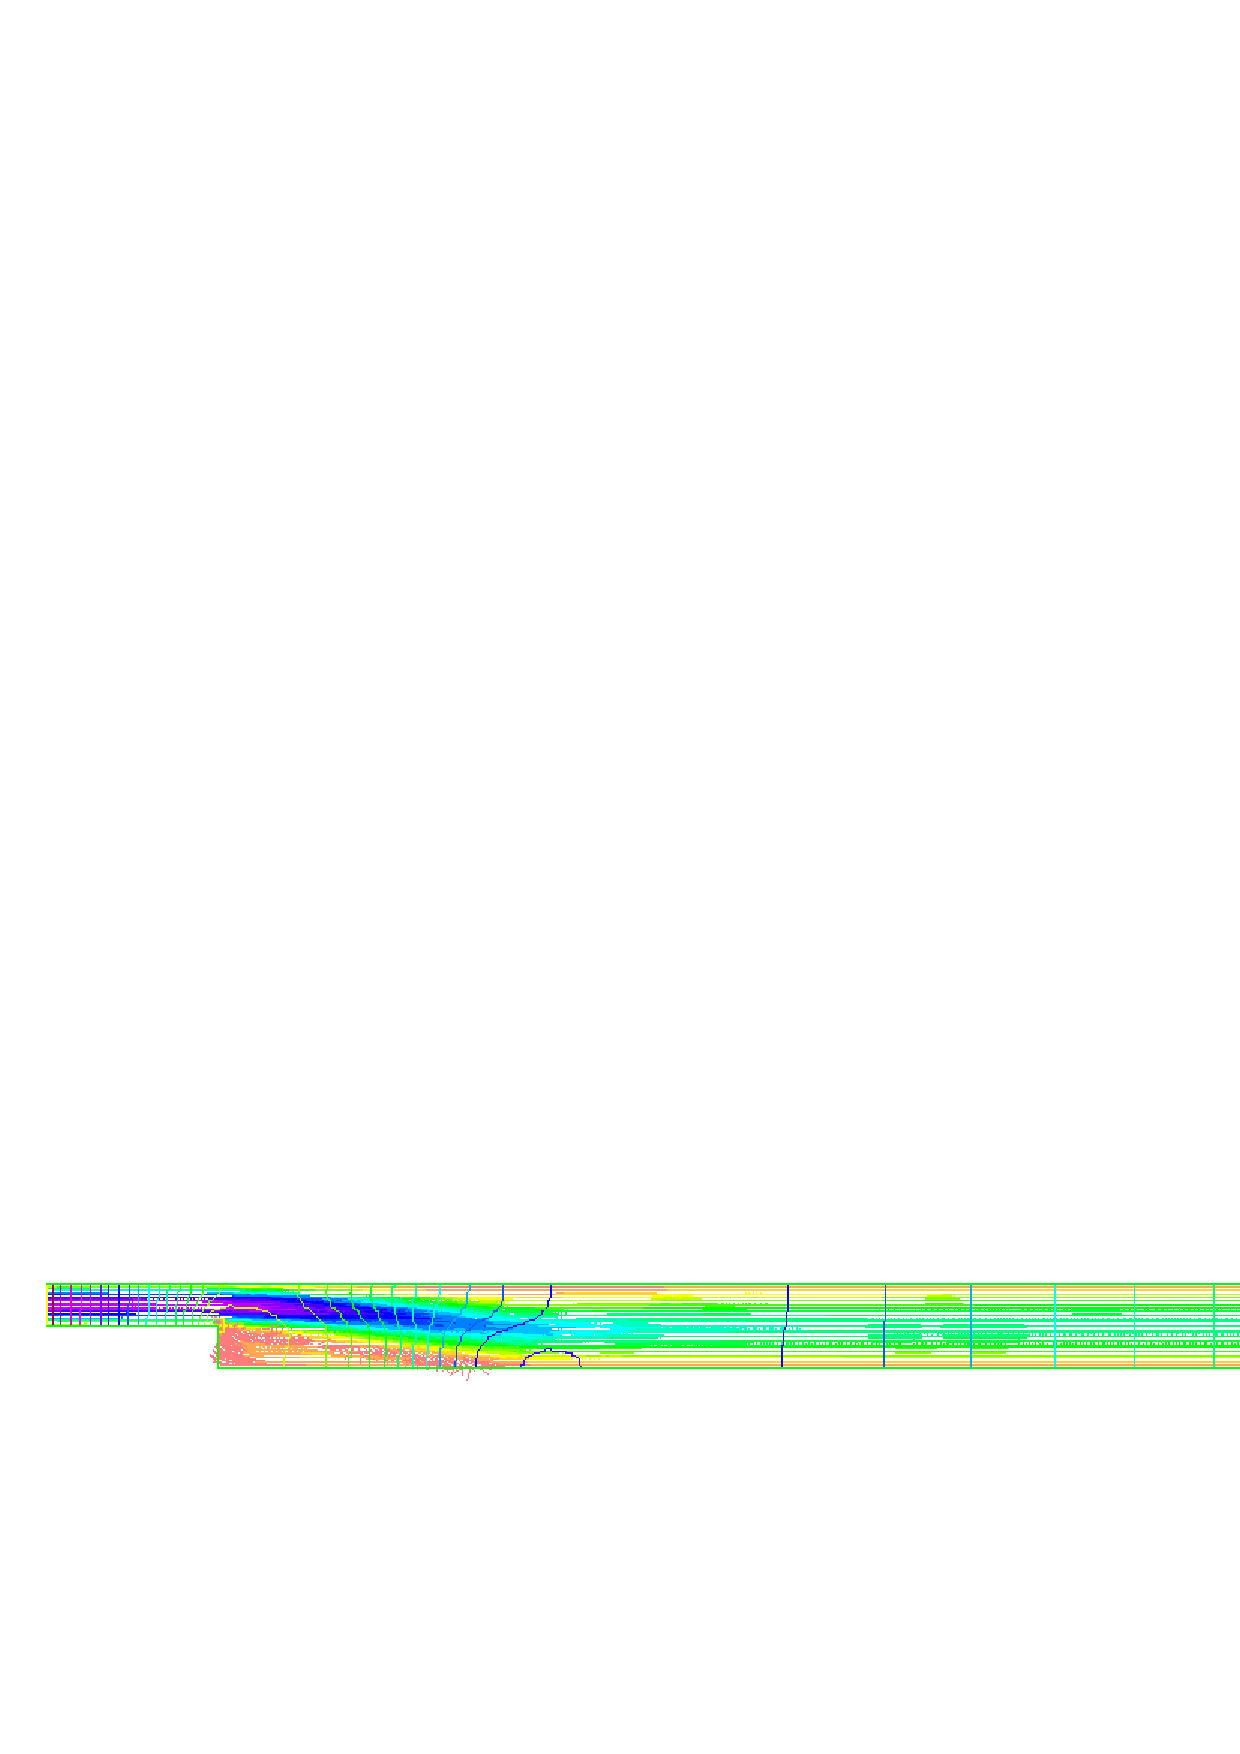
\includegraphics[scale=0.30]{Sol1}
 \caption{Solution C++}
\end{figure}
\end{center}

\begin{center}
\begin{figure}[h]
 \centering
 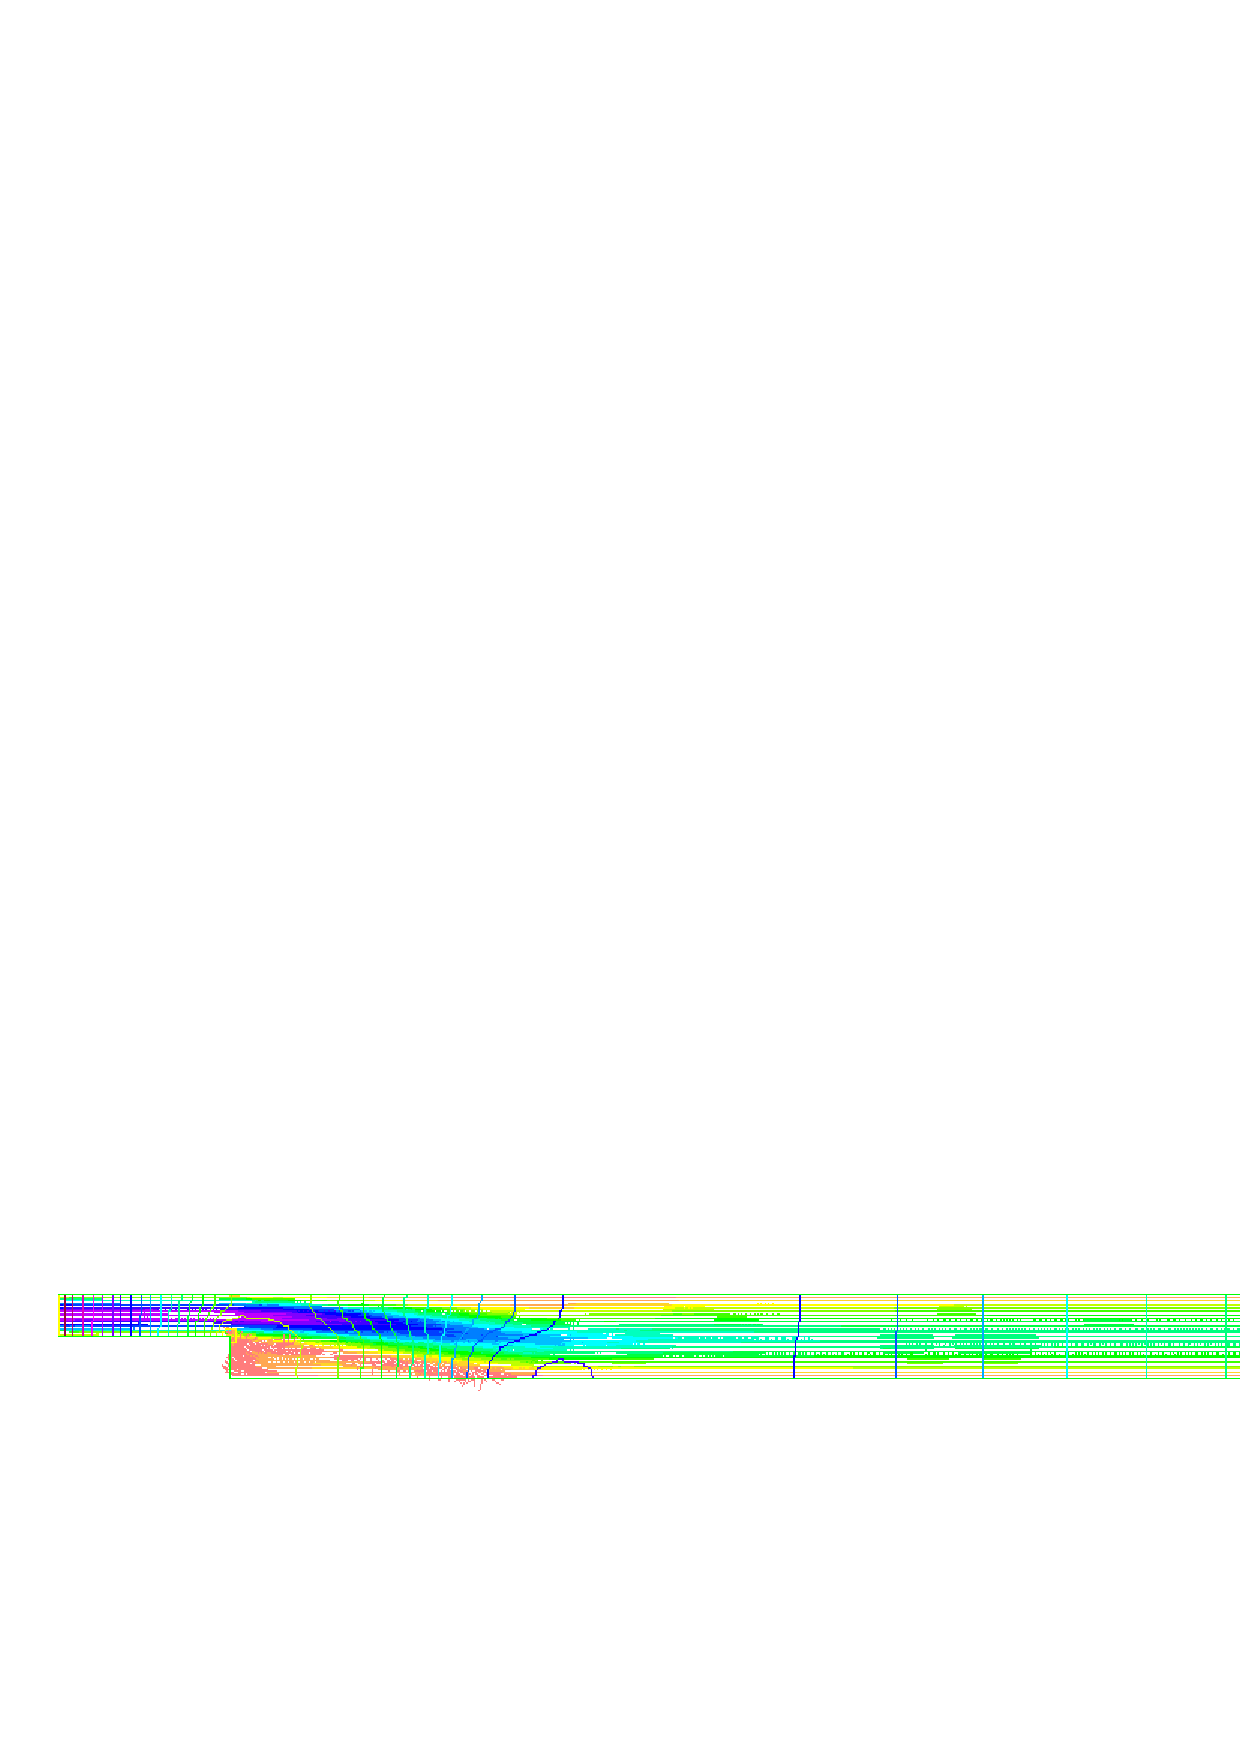
\includegraphics[scale=0.30]{Sol2}
 \caption{Solution FF++}
\end{figure}
\end{center}

\begin{center}
\begin{figure}[h]
 \centering
 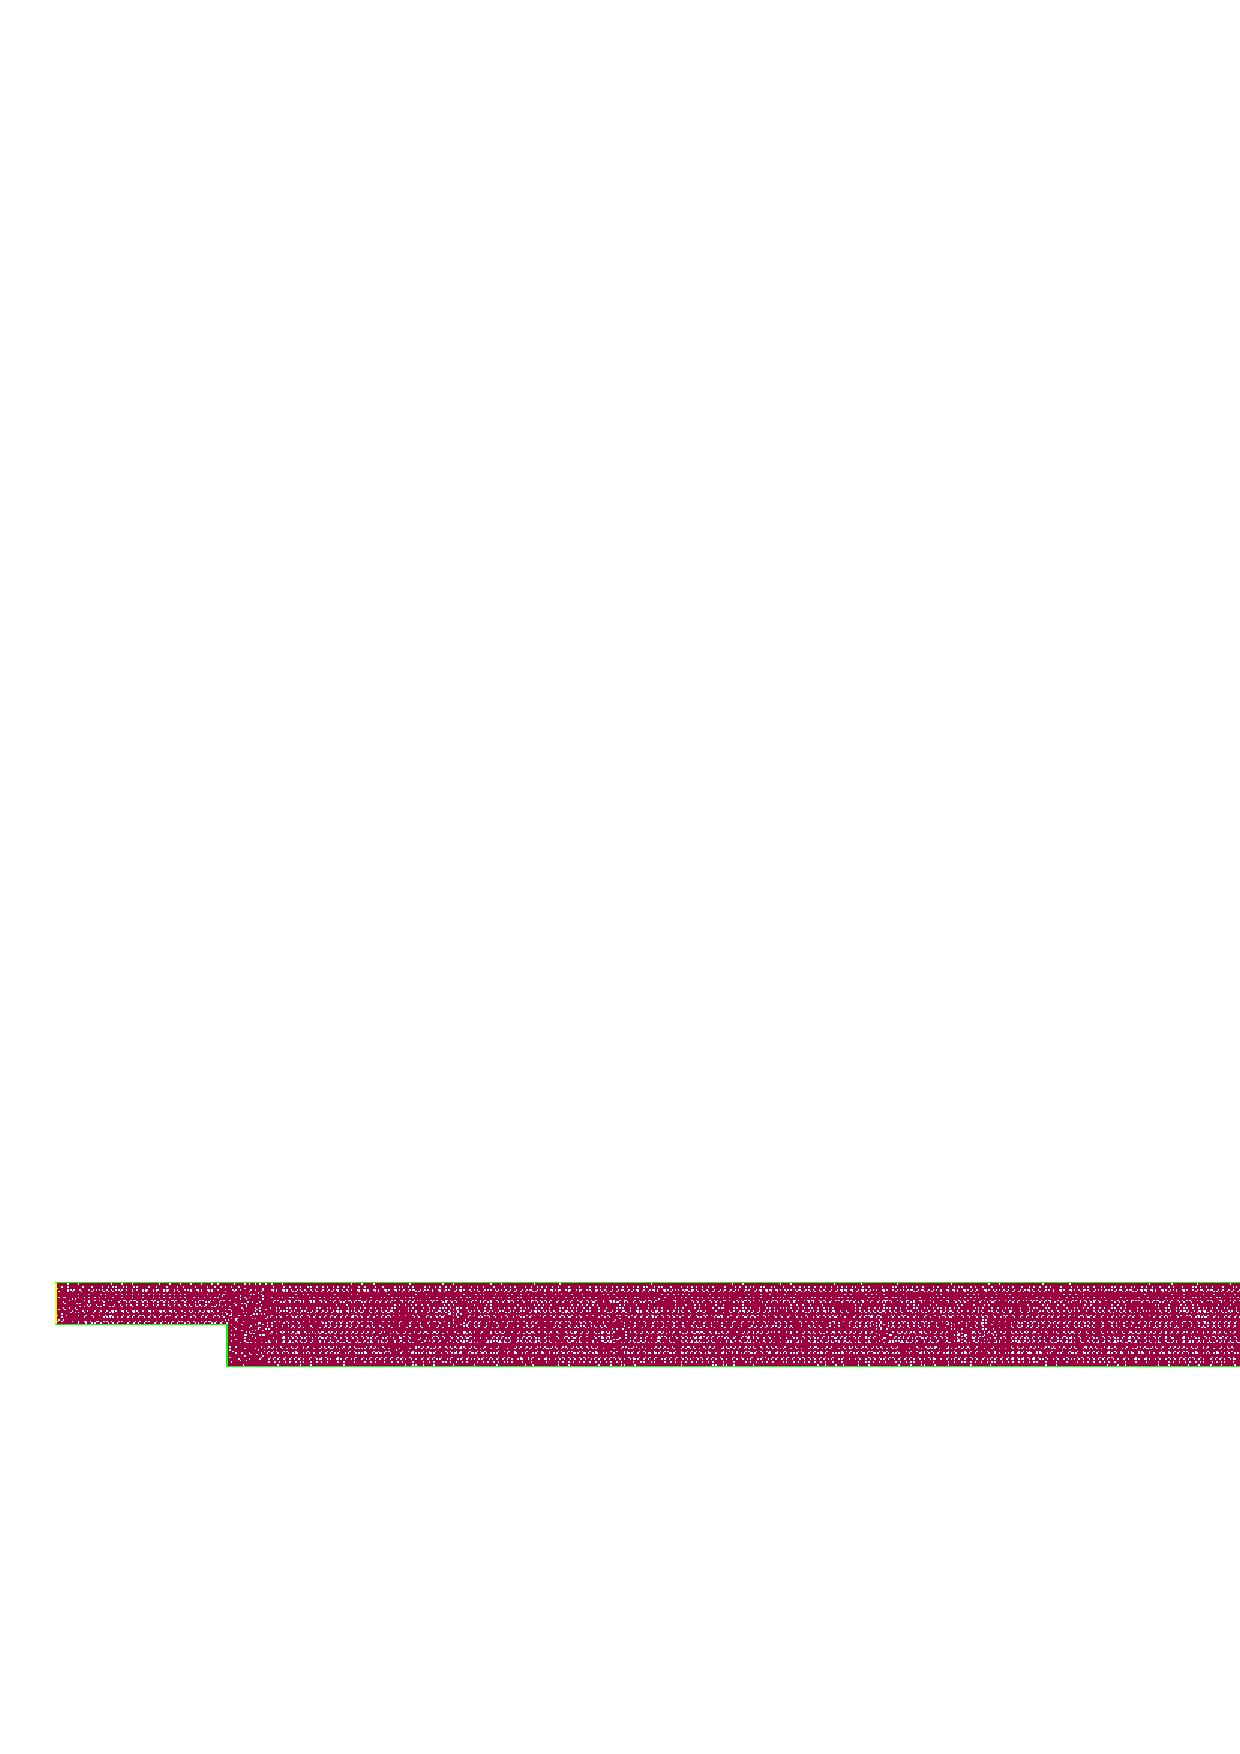
\includegraphics[scale=0.30]{Erreur}
 \caption{Différence C++ FF++}
\end{figure}
\end{center} 
%%%%%%%%%%%%%%%%%%%%%STRUCTURE ET UTILISATION %%%%%%%%%%%%%%%%%%
%%%%%%%%%%%%%%%%%%%%%%%%%%%%%%%%%%%%%%%%%%%%%%%%%%%%%%%%%%%%%%%%%%%%%%%%%%%%%%%%%%%%%%%%%
%=======================================================================================%
%%%%%%%%%%%%%%%%%%%%%%%%%%%%%%%%%%%%%%%%%%%%%%%%%%%%%%%%%%%%%%%%%%%%%%%%%%%%%%%%%%%%%%%%%
\chapter{Qt Programmation GUI}
Qt est un framework C++ permettant de développer des applications GUI multiplates-formes. Qt permet aux programmeurs d'employer une seule arborescence source pour des application qui s'éxécuteront sous Windows, Mac OS X, Linux et de nombreuses autres versions d'Unix avec X11. Les bibliothèques et outils Qt font également partie de Qtopia Core. J'ai l'idée de programmation Qt quand je suis tombé sur le siteweb :
\begin{itemize}
 \item Introduction : \href{http://www.siteduzero.com/tutoriel-3-11240-introduction-a-qt.html}{http://www.siteduzero.com/tutoriel-3-11240-introduction-a-qt.html}
\end{itemize}
qui est une très bonne introduction �  la programmation Qt. Ensuite, on peut consulter les sites officiels pour une pratique et compréhension plus approfondie :
\begin{itemize}
 \item Documentation [fr] : \href{http://doc.qtfr.org/}{http://doc.qtfr.org/}
 \item Documentation [en] : \href{http://doc.trolltech.com/}{http://doc.trolltech.com/}
\end{itemize}
Pour apprendre Qt, j'ai consulté en premier l'introduction sur le siteduzéro pour comprendre la compilation, l'installation de Qt. Ensuite, je suis parti sur le site officielle pour télécharger les exemples, les compiler et les corriger pour approfondir. Pour une lecture plus structurée, on pourra consulter \cite{NCT7}
%%%%%%%%%%%%%%%%%%%%%%% PRÉSENTATION GUI_NS %%%%%%%%%%%%%%%%%%%%%%%%%%%%% 
\section{Présentation du GUI\_NS}
Mon programme GUI\_NS se compose principalement des objets QLineEdit, QPushButton, QProcess. Les QLineEdit permet de saisir un texte, c'est l�  que l'utilisateur fait entrer ses données désirées. QPushButton est simplement un ... bouton. QProcess est comme un processu, fait tourner des programmes extérieurs. Le mécanisme général est �  chaque fois qu'on presse sur un Bouton, il émet un signal, qui fait appel �  \"quelques choses\".Celles-ci peut être d'appel une fonction, démarrer un processu, déclencher le chronomètre, lire les données dans les champs, écrire les données dans les champs, dans les fichiers..ect...Ce mécanisme se réalise grâce �  la méthode statique  QObject::connect(Objet1,SIGNAL(...),Objet2,SLOT(...)). 
\paragraph{Fenetre Creat Mesh :} 
\begin{center}
\begin{figure}[h]
 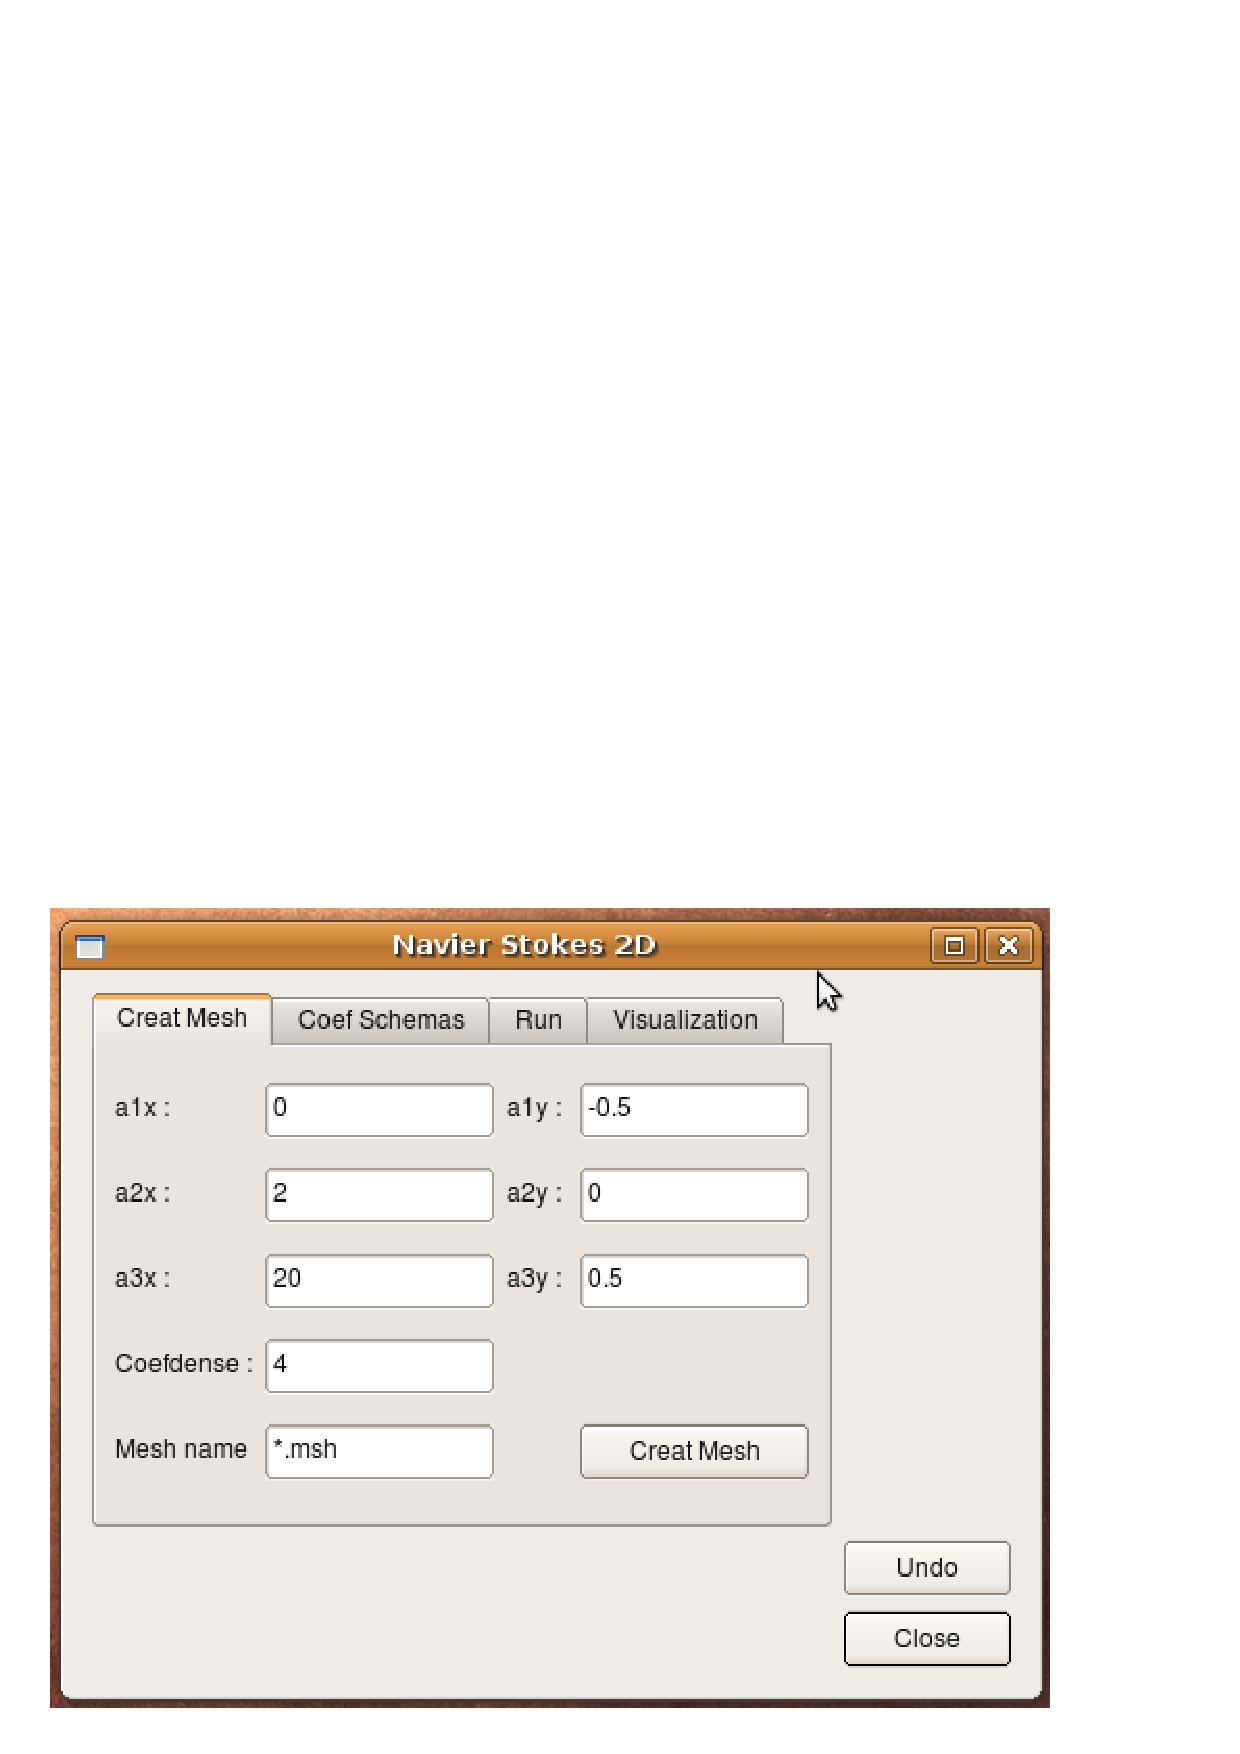
\includegraphics[scale=0.60]{CreatMesh}
 \caption{Fênetre Creat Mesh} 
\end{figure}
\end{center}
Dans cette fenetre, on a la connection :
\begin{lstlisting}
  QObject::connect(button_CreatMesh,SIGNAL(clicked()),
                   this,SLOT(CreatMeshSLOT()));
\end{lstlisting}
qui fait que si je clike sur le bouton CreatMesh, la fonction spéciale (SLOT) CreatMeshSLOT() sera appelée, elle lit les données dans les champs saisies, les écrit dans le fichier MeshCorner.txt, appelle le script CreatMesh.edp :
\begin{lstlisting}
void  CreatMeshTab::CreatMeshSLOT(){
  system("rm -f *.msh");
  double a1x_value=LineEdita1x->text().toDouble();
  double a1y_value=LineEdita1y->text().toDouble();
  double a2x_value=LineEdita2x->text().toDouble();
  double a2y_value=LineEdita2y->text().toDouble();
  double a3x_value=LineEdita3x->text().toDouble();
  double a3y_value=LineEdita3y->text().toDouble();
  int Coefdense_value=LineEditCoefdense->text().toInt();
  {
    ofstream fileout("MeshCorner.txt");
    fileout<<a1x_value<<" "<<a1y_value<<endl
	   <<a2x_value<<" "<<a2y_value<<endl
	   <<a3x_value<<" "<<a3y_value<<endl
	   <<Coefdense_value<<endl;
  }
  system("FreeFem++ CreatMesh.edp");
  char commandeSaveMesh[256];
  strcpy(commandeSaveMesh,"mv MyMesh.msh ");
  strcat(commandeSaveMesh,
        LineEditNameMeshSave->text().toStdString().c_str());
  system(commandeSaveMesh);
  //cout<<commandeSaveMesh<<endl;
} 
\end{lstlisting}
\paragraph{Fenetre Coef Schemas :}
\begin{center}
\begin{figure}[h]
 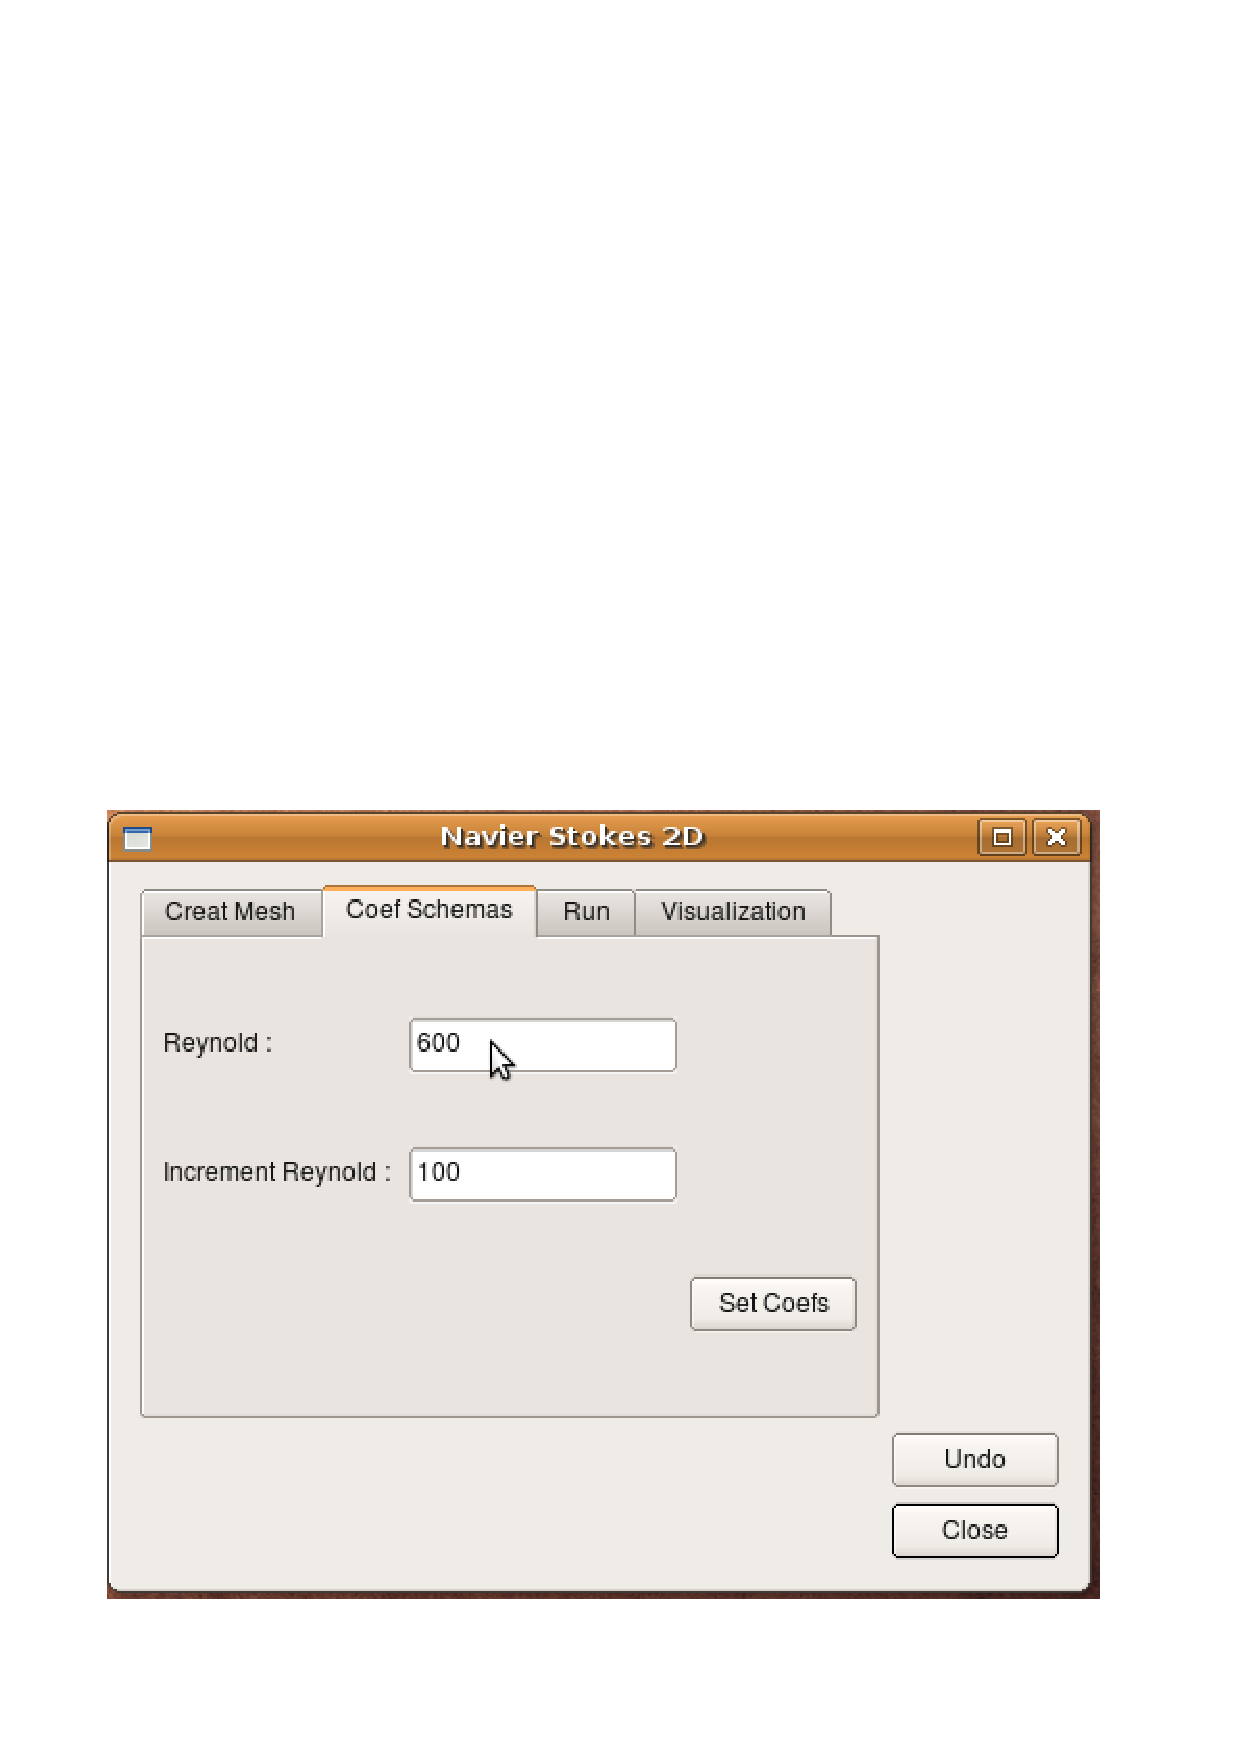
\includegraphics[scale=0.50]{CoefSchema}
 \caption{Fênetre Coef Schéma} 
\end{figure}
\end{center}
De même, la fenetre Coef Schéma a pour connection :
\begin{lstlisting}
QObject::connect(button_SetCoef,SIGNAL(clicked()),
                 this,SLOT(SetCoefSLOT())); 
\end{lstlisting}
En appuyant sur le bouton \textbf{Set Coef}, on écrit ces données dans le fichier CoefSchemas.txt et modifie les données dans la fenetre Run.
\paragraph{Fenetre Run :}
\begin{center}
\begin{figure}[h]
 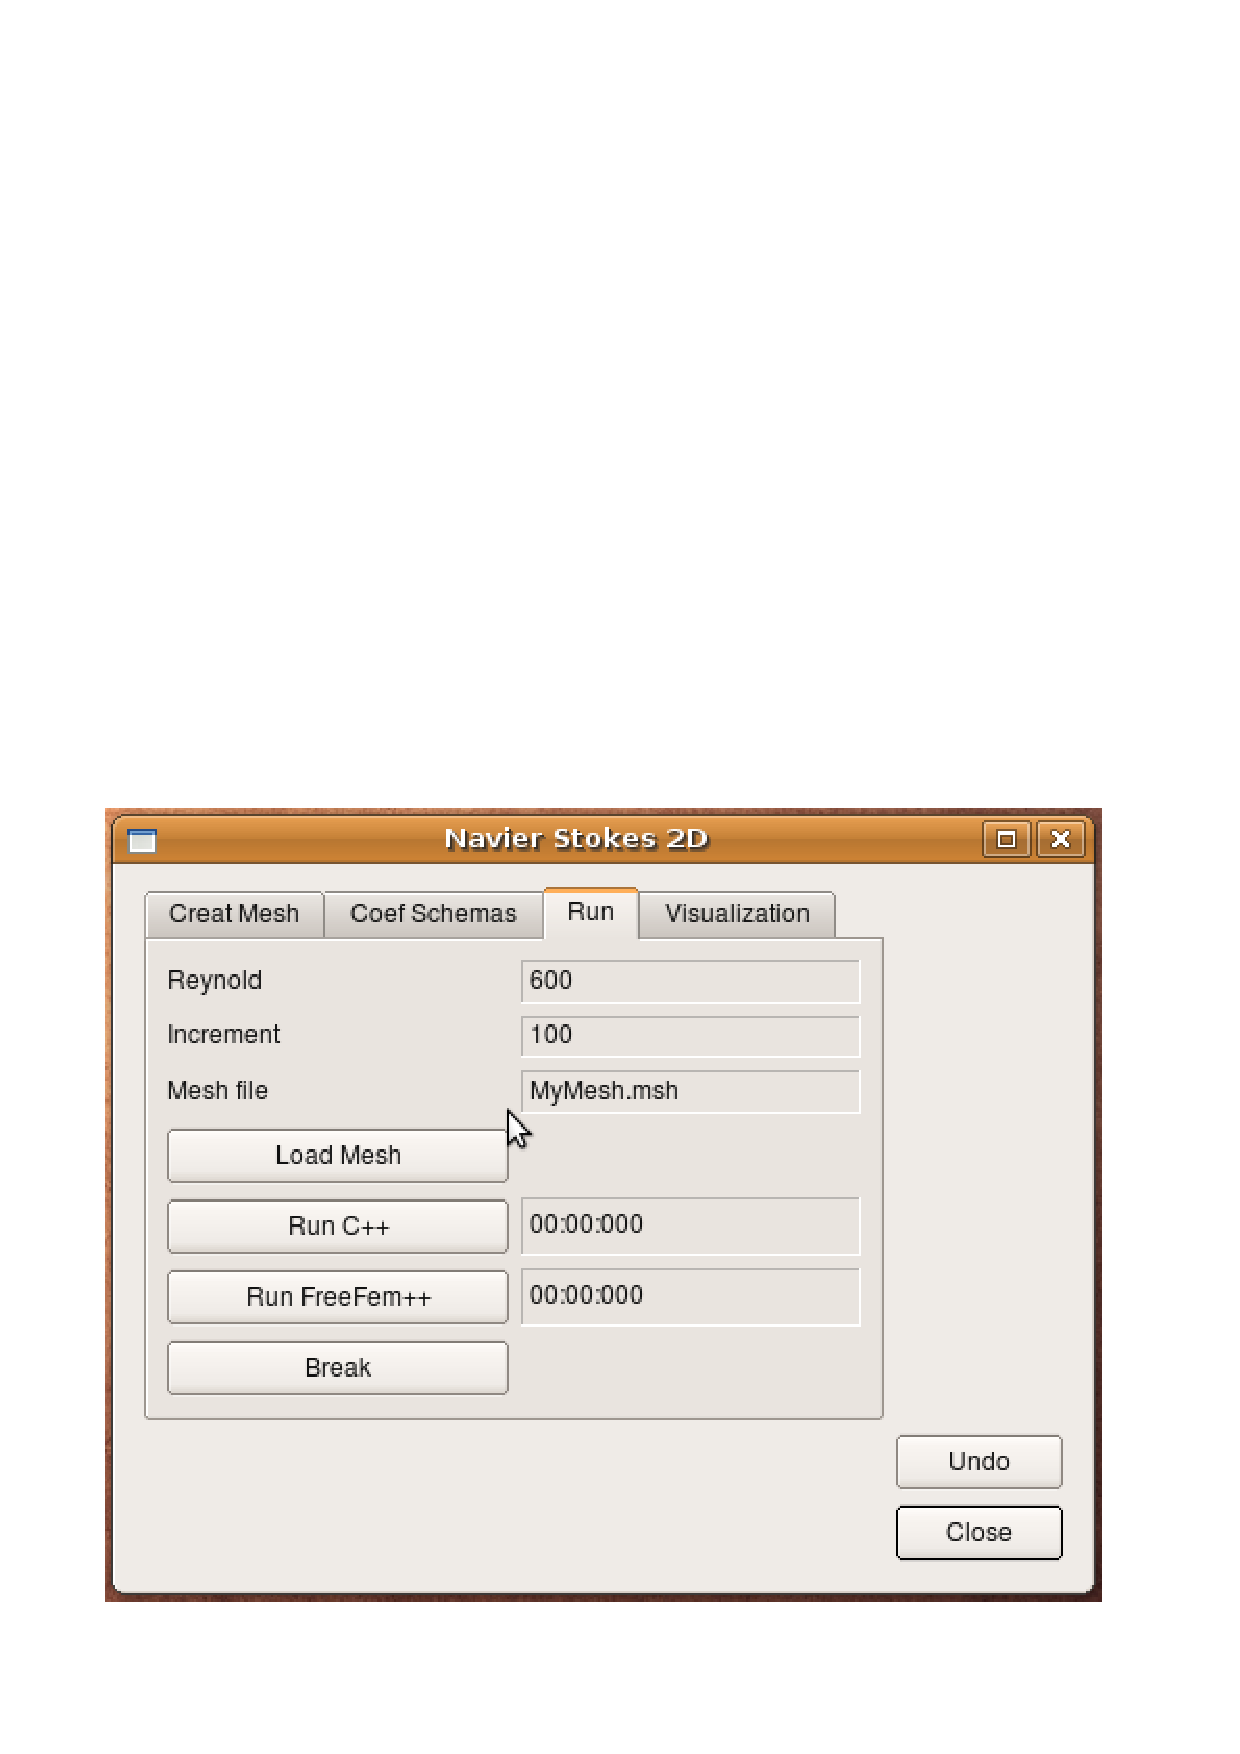
\includegraphics[scale=0.50]{Run}
 \caption{Fênetre Run} 
\end{figure}
\end{center}
La fenetre Run est la plus compliquée, contient :
\begin{lstlisting}
QObject::connect(TimerChronoCpp,SIGNAL(timeout()),
                 this,SLOT(UpdateTimeCppSLOT()));
QObject::connect(TimerChronoFFpp,SIGNAL(timeout()),
                 this,SLOT(UpdateTimeFFppSLOT()));
QObject::connect(RunProcess,SIGNAL(finished(int,QProcess::ExitStatus)),
                 TimerChronoCpp,SLOT(stop()));
QObject::connect(RunProcess,SIGNAL(finished(int,QProcess::ExitStatus)),
                 TimerChronoFFpp,SLOT(stop()));
QObject::connect(button_LoadMesh,SIGNAL(clicked()),
                 this,SLOT(LoadMeshSLOT()));
QObject::connect(button_RunCpp,SIGNAL(clicked()),
                 RunProcess,SLOT(kill()));
QObject::connect(button_RunCpp,SIGNAL(clicked()),
                 this,SLOT(RunCppSLOT()));
QObject::connect(button_RunFFpp,SIGNAL(clicked()),
                 RunProcess,SLOT(kill()));
QObject::connect(button_RunFFpp,SIGNAL(clicked()),
                 this,SLOT(RunFFppSLOT()));
QObject::connect(button_Break,SIGNAL(clicked()),
                 RunProcess,SLOT(kill()));
QObject::connect(button_Break,SIGNAL(clicked()),
                 this,SLOT(ResetTimeSLOT()));
\end{lstlisting}
Le bouton \textbf{Load Mesh} recherche le fichier de maillage, modifie le text dans le champs Mesh file. Le bouton \textbf{Run C++} appelle le programme C++, déclanche le chronomètre Cpp. Le bouton \textbf{Run FreeFem++} appelle le programme FF++, déclanche le chronomètre FFpp. Le bouton \textbf{Break} arrête tout programme de façon brutale et remet le chronomètre �  zéro.
\paragraph{Fenetre Visualization :}
\begin{center}
\begin{figure}[h]
 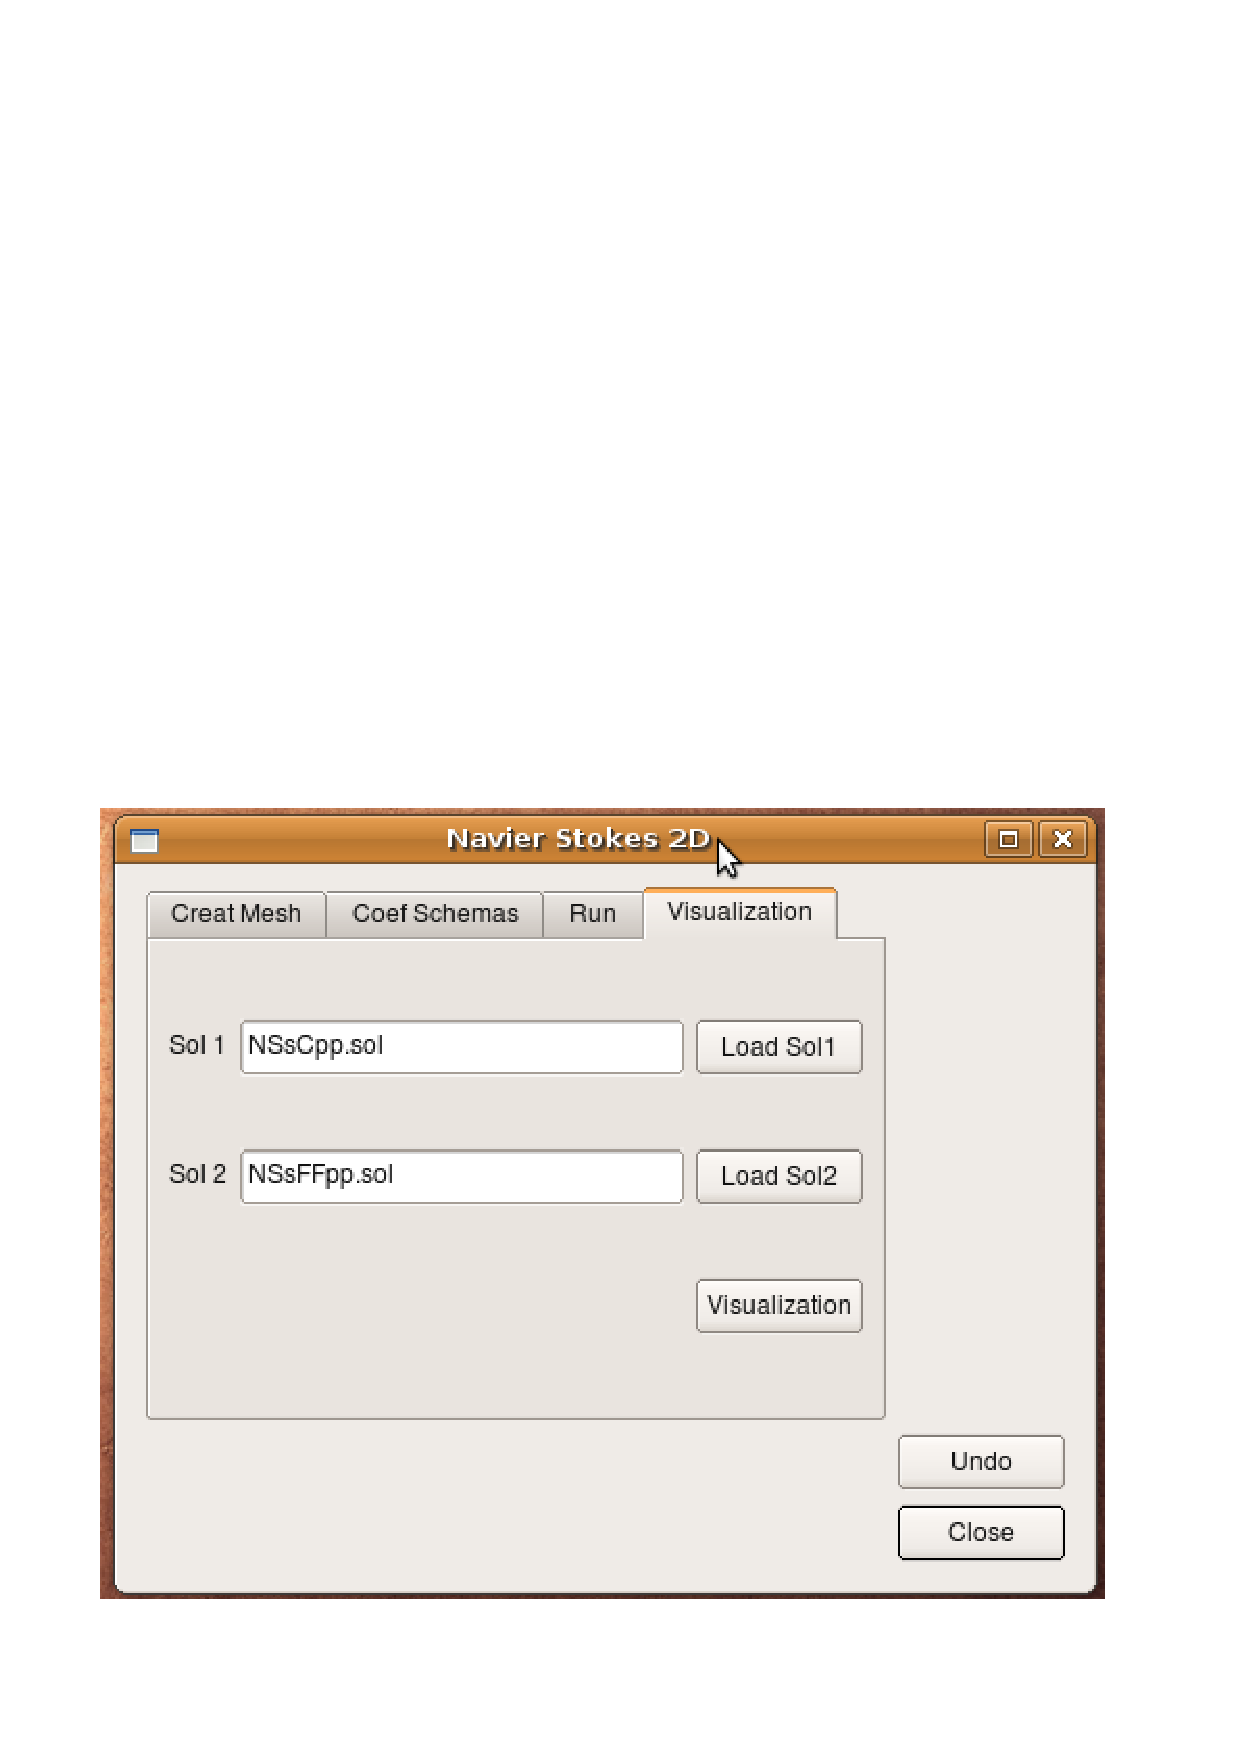
\includegraphics[scale=0.50]{Visualization}
 \caption{Fenetre Visualisation} 
\end{figure}
\end{center}
Cette fênetre est aussi simple que la fenetre Coef Schéma, qui lit les fichiers de solution, appelle le programme C++ ./visualisation (qui crée encore un script FreeFem++) pour visualiser les solutions. Le bouton \textbf{Load Sol1} recherche la première solution �  visualiser. Le bouton \textbf{Load Sol2} recherche la deuxième solution �  visualiser. Le bouton \textbf{Visualization} appelle le programme :
\begin{lstlisting}
Prompt$ ./Visualization First.sol Second.sol 
\end{lstlisting}
Si on ne met rien dans le champs saisie de la deuxième solution, \textbf{Visualization} appelle :
\begin{lstlisting}
Prompt$ ./Visualization First.sol 
\end{lstlisting}
\begin{lstlisting}
QObject::connect(button_LoadSol1,SIGNAL(clicked()),
                 this,SLOT(LoadSol1SLOT()));
QObject::connect(button_LoadSol2,SIGNAL(clicked()),
                 this,SLOT(LoadSol2SLOT()));
QObject::connect(button_Visualization,SIGNAL(clicked()),
                 this,SLOT(VisualizationSLOT()));
\end{lstlisting}
\paragraph{Remarque sur QProcess:}
Quelques SLOT fait appel aux programme externe sous forme processu. Pour ne pas s'occuper des iostandard du programme externe, il faut le regler en mode spécifique utilisant la fonction setProcessChannelMode(mode) de la classe QProcess.
\begin{lstlisting}
Process::setProcessChannelMode(QProcess::ForwardedChannels);
\end{lstlisting}
\paragraph{Remarque sur QTime et QTimer:}
Pour la construction de l'horloge de calcul, il faut deux objets qui se ressemble en notation QTime et QTimer. Ces deux objets sont utilisé pour de buts différents QTime s'utilise comme une horloge, tandis que QTimer s'utiliser comme un chronomètre :
\begin{lstlisting}
QTime *Chronometre;QTime *TempsCalcul;
QTimer *TimerChronoCpp;QTimer *TimerChronoFFpp;
\end{lstlisting}
TimerChronoCpp, TimerChronoFFpp sont utilisés pour chronomètrer les durées de calcul respectivement de C++ et FF++. Ensuite, en utilisant la fonction de QTime::elapsed(), on peut calculer le temps écoulé souhaité.
%%%%%%%%%%%%%%%%%%%%%%% PRÉSENTATION GUI_NS %%%%%%%%%%%%%%%%%%%%%%%%%%%%% 

%%%%%%%%%%%%%%%%%%%%%%% Utilisation GUI_NS %%%%%%%%%%%%%%%%%%%%%%%%%%%%% 
\section{Utilisation}
La complilation est assez compliquée utilisant un outil spécifique : qmake. Cet outil génère automatiquement le fichier Makefile pour le projet. Pour cette raison, il faut mettre le programme dans un directoire différent que le projet principale, le compiler, et l'amener dans le projet après la compilation pour l'utiliser. 
%%%%%%%%%%%%%%%%%%%%%%% Utilisation GUI_NS %%%%%%%%%%%%%%%%%%%%%%%%%%%%% 





\bibliography{ReferenceNCT}
\nocite{*}
\end{document}



